\documentclass[10 pt]{beamer}
\usepackage[utf8]{inputenc}
%\usepackage[latin1]{inputenc}
%\usepackage[cyr]{aeguill}
\usepackage[T1]{fontenc}
\usepackage{graphicx}
\usepackage{amsmath,amsfonts,amsthm,amssymb}
\usepackage{algorithm}
\usepackage{algorithmic}
%\usepackage[]{algorithm2e}
\usepackage{hyperref}
\usepackage{color}
\usepackage{pstricks}
%\usepackage{stmaryrd}
%\usepackage{enumitem} 
\usepackage{bm}
\usepackage{array}
\usepackage{relsize,exscale}
\usepackage{caption}
\usepackage{subcaption}
%\usepackage{tikz}
%\usetikzlibrary{calc}
\DeclareMathOperator*{\argmin}{argmin}
\definecolor{ao(english)}{rgb}{0.0, 0.5, 0.0}
\definecolor{armygreen}{rgb}{0.29, 0.33, 0.13}
\definecolor{britishracinggreen}{rgb}{0.0, 0.26, 0.15}
\definecolor{cadmiumgreen}{rgb}{0.0, 0.42, 0.24}
\definecolor{indigo}{rgb}{0.29, 0.0, 0.51}
\definecolor{lightgray}{gray}{0.85}
\definecolor{midnightblue}{rgb}{0.1, 0.1, 0.44}
\definecolor{burntorange}{rgb}{0.8, 0.33, 0.0}
\definecolor{royalblue}{rgb}{0.25, 0.41, 0.88}
\definecolor{darkmagenta}{rgb}{0.55, 0.0, 0.55}
\definecolor{byzantine}{rgb}{0.74, 0.2, 0.64}
\definecolor{blue-violet}{rgb}{0.54, 0.17, 0.89}
\definecolor{brown-traditional}{rgb}{0.59, 0.29, 0.0}
\definecolor{brown-web}{rgb}{0.65, 0.16, 0.16}
\definecolor{burgundy}{rgb}{0.5, 0.0, 0.13}
\definecolor{electricpurple}{rgb}{0.75, 0.0, 1.0}
\definecolor{gray}{rgb}{0.5, 0.5, 0.5}
\definecolor{goldenbrown}{rgb}{0.6, 0.4, 0.08}
\definecolor{armygreen}{rgb}{0.29, 0.33, 0.13}
\definecolor{calpolypomonagreen}{rgb}{0.12, 0.3, 0.17}
\definecolor{caputmortuum}{rgb}{0.35, 0.15, 0.13}
\definecolor{carmine}{rgb}{0.59, 0.0, 0.09}
\definecolor{chocolate-traditional}{rgb}{0.48, 0.25, 0.0}
\definecolor{lincolngreen}{rgb}{0.11, 0.35, 0.02}
\definecolor{magenta}{rgb}{1.0, 0.0, 1.0}
\definecolor{auburn}{rgb}{0.43, 0.21, 0.1}
\definecolor{bole}{rgb}{0.47, 0.27, 0.23}
 	\definecolor{bulgarianrose}{rgb}{0.28, 0.02, 0.03}
%\usepackage[dvipsnames]{xcolor}
%\xdefinecolor{vert_olive}{named}{OliveGreen}
%\xdefinecolor{bleuviolet}{named}{BlueViolet}
%\xdefinecolor{bleucadet}{named}{CadetBlue}
%\xdefinecolor{bleunuit}{named}{MidnightBlue}
\graphicspath{{./Figures/}}

\renewcommand{\div}{\mathrm{div}}
\usepackage{graphicx} 
\usepackage{epstopdf}

\usetheme{Frankfurt}

\title[Enumath 2017]{Adaptive inexact semi-smooth Newton methods for a contact between two membranes}
\author[Jad Dabaghi]{\underline{Jad Dabaghi}, Vincent Martin, Martin Vohral\'ik}
\institute[]{Inria Paris \& Université Paris-Est}
\date{Voss, September 25 2017}
\subject{Numerical Analysis}
\newcommand{\nc}{\newcommand}

%%%%commandes principales

%\newtheorem{theorem}{Theorem}
\newtheorem{lemme}{Lemma}
%\newtheorem{definition}{Definition}
\newtheorem{proposition}
{Proposition}
\newtheorem{notation}{Notation}
\newtheorem{remarque}
{Remark}
\newtheorem{assumption}{Assumption}
%\newtheorem{corollary}{Corollary}


%%%%commandes principales



\nc{\myth}[1]{#1^{\scriptsize\mbox{th}}}
\nc{\lth}{\myth{l}}
\nc{\ith}{\myth{i}}
\nc{\dps}{\displaystyle}
\newcommand{\cf}{{\it cf.}}
\nc{\card}{card \hspace {0.2cm}}
\nc{\tq}{{t.q}}
\renewcommand{\div}{\mathrm{div\,}}


\newcommand{\TODO}[1]{{\red{\bf!!! \`A faire~: #1!!!}}}
\nc{\TODOJAD}[1]{{\red{\bf \'A faire~: #1}}}
\newcommand{\modifVct}[1]{\textcolor{royalblue}{#1}}


%%%%commandes ensembles entiers naturels, réels

\newcommand{\matR}{\ensuremath{\mathbb{R}}}
\newcommand{\matN}{\ensuremath{\mathbb{N}}}
\newcommand{\matZ}{\ensuremath{\mathbb{Z}}}
\newcommand{\matX}{\ensuremath{\mathbb{X}}}

%%%%%%

\newcommand{\vv}[1]{\ensuremath{{\bf #1}}}
\newcommand{\vu}{\vv{u}}

\newcommand{\dd}{\ensuremath{\mathrm{dt}}}
\newcommand\eal{{\em et al.}}

%%%%% Flux de fick




\nc{\CFun}{{\bf C}}
\nc{\JacMat}[1]{{\bf J}_{#1}}
\nc{\JacCFun}{\JacMat{\CFun}}



%%%%notations maillages

\nc{\Eh}{\mathcal{E}_h}
\nc{\Vhint}{\mathcal{V}_h^{\mathrm{int}}}
\nc{\Vjint}{\mathcal{V}_j^{\mathrm{int}}}
\nc{\VK}{\mathcal{V}_K}
\nc{\Vhext}{\mathcal{V}_h^{\mathrm{ext}}}
\nc{\Vhiint}{\mathcal{V}_{j-1}^{\mathrm{int}}}
\nc{\Vhintprime}{\mathcal{V}_{h}^{int}}
\nc{\Vhiipriment}{\mathcal{V}_{h-1}^{int}}
\nc{\Th}{\mathcal{T}_h}
\nc{\Tl}{\mathcal{T}_l}
\nc{\Tj}{\mathcal{T}_j}
\nc{\tauunha}{{\bm{\mathcal{\tau}}}_{1h}^{\ba}}
\nc{\taudeuxha}{{\bm{\mathcal{\tau}}}_{2h}^{\ba}}
\nc{\guna}{g_{\mathrm{1}}^{\ba}}
\nc{\gdeuxa}{g_{\mathrm{2}}^{\ba}}

\nc{\Ehint}{\mathcal{E}_h^{int}}
\nc{\Ehext}{\mathcal{E}_h^{ext}}
\nc{\Vh}{\mathcal{V}_h}
\nc{\ba}{{\bm a}}
\nc{\bal}{{\bm a_l}}
\nc{\baprime}{{\bm a'}}
\nc{\oma}{\omega_{\bm a}}

%%%inconnues discrètes, linéarisés, muligrille

\nc{\bu}{{\bm u}}
\nc{\bU}{{\bm U}}
\nc{\bUk}{{\bm U}^k}
\nc{\bUki}{{\bm U}^{k,i}}
\nc{\bRki}{{\bm R}^{k,i}}

\nc{\bF}{{\bm F}}
\nc{\bB}{{\bm B}}
\nc{\bC}{{\bm C}}
\nc{\bb}{{\bm b}}
\nc{\bS}{{\bm S}}
\nc{\bK}{{\bm K}}
\nc{\bD}{{\bm D}}
\nc{\bH}{{\bm H}}
\nc{\bG}{{\bm G}}
\nc{\bR}{{\bm R}}
\nc{\bs}{{\bm s}}
\nc{\bw}{{\bm w}}
\nc{\uh}{{\bm u}_h}
\nc{\bv}{{\bm v}}
\nc{\bXunh}{{\bm X}_{1h}}
\nc{\bXunhki}{{\bm X}_{1h}^{k,i}}
\nc{\bXdeuxh}{{\bm X}_{2h}}
\nc{\bXdeuxhki}{{\bm X}_{2h}^{k,i}}
\nc{\bXtroish}{{\bm X}_{3h}}
\nc{\bXtroishki}{{\bm X}_{3h}^{k,i}}
\nc{\X}{{\bf X}}
\nc{\Xh}{{\bf X}_h}
\nc{\bh}{{\bm b}_h}
\nc{\rhk}{{\bm r}_h^k}
\nc{\rhki}{{\bm r}_h^{k,i}}
\nc{\rhkimoinsun}{{\bm r}_h^{k,i-1}}
\nc{\runhkimoinsun}{{\bm r}_{1h}^{k,i-1}}
\nc{\runJkimoinsun}{{\bm r}_{1J}^{k,i-1}}
\nc{\rHk}{{\bm r}_H^k}
\nc{\rhi}{{\bm r}_h^i}
\nc{\rHi}{{\bm r}_H^i}
\nc{\rdeuxhkimoinsun}{{\bm r}_{2h}^{k,i-1}}

\nc{\rdeuxJkimoinsun}{{\bm r}_{2J}^{k,i-1}}

\nc{\Xhki}{{\bf X}_h^{\textcolor{royalblue}{k},\textcolor{burntorange}{i}}}
\nc{\Xhkii}{{\bf X}_h^{k,i-1}}
\nc{\Xhk}{{\bf X}_h^{\textcolor{royalblue}{k}}}
\nc{\Runhki}{{\bm R}_{1h}^{\textcolor{royalblue}{k},\textcolor{burntorange}{i}}}
\nc{\Rdeuxhki}{{\bm R}_{2h}^{\textcolor{royalblue}{k},\textcolor{burntorange}{i}}}

\nc{\runa}{r_1^{\ba}}
\nc{\rdeuxa}{r_2^{\ba}}

\nc{\uhk}{{\bm u}^{k}_h}

\nc{\ujhk}{u^{k}_{jh}}

\nc{\uhki}{{\bm u}^{{\textcolor{royalblue}{k},\textcolor{burntorange}{i}}}_h}
\nc{\ujhki}{u^{k,i}_{jh}}

\nc{\uunhk}{u_{1h}^{\textcolor{royalblue}{k}}}

\nc{\udeuxhk}{u_{2h}^{\textcolor{royalblue}{k}}}

\nc{\uunhki}{u_{1h}^{\textcolor{royalblue}{k},\textcolor{burntorange}{i}}}
\nc{\uunhprimeki}{u^{k,i}_{1h'}}

\nc{\uun}{u_1}
\nc{\udeux}{u_2}


\nc{\uununki}{u^{k,i}_{11}}


\nc{\uunhkimoinsun}{u^{k,i-1}_{1h}}
\nc{\udeuxhki}{u_{2h}^{\textcolor{royalblue}{k},\textcolor{burntorange}{i}}}

\nc{\udeuxhprimeki}{u^{k,i}_{2h'}}


\nc{\udeuxunki}{u^{k,i}_{21}}

\nc{\udeuxhkimoinsun}{u^{k,i-1}_{2h}}

\nc{\uunhkmoinsun}{u^{k-1}_{1h}}
\nc{\udeuxhkmoinsun}{u^{k-1}_{2h}}

\nc{\uunhzero}{u_{1h}^0}
\nc{\udeuxhzero}{u_{2h}^0}
\nc{\uunhzeroki}{u^{0,k,i}_{1h}}
\nc{\uunhzerokmoinsun}{u^{0,k-1}_{1h}}
\nc{\uunhzerokimoinsun}{u^{0,k,i-1}_{1h}}

\nc{\ghtilde}{{\tilde{g}}_h}



\nc{\Xk}{{\bf X}^k}

%%%% flux discret
\nc{\sigunha}{{\bm{\sigma}}_{1h}^{\ba}}
\nc{\sigdeuxha}{{\bm{\sigma}}_{2h}^{\ba}}


%%\nc{\rhki}{{\bf r}_h^{k,i}}
\nc{\Rhki}{{\bm R}_h^{\textcolor{royalblue}{k},\textcolor{burntorange}{i}}}
\nc{\Rhkimoinsunal}{{\bm R}_{h}^{k,i-1}(\ba_l)}
\nc{\Rhmoinsunkimoinsunal}{{\bm R}_{h-1}^{k,i-1}(\ba_l)}

\nc{\Rmhmoinsunkimoinsunal}{{\bm R}_{m,h-1}^{k,i-1}(\ba_l)}
\nc{\Runhmoinsunkimoinsunal}{{\bm R}_{1,h-1}^{k,i-1}(\ba_l)}

\nc{\RunJmoinsunkimoinsunal}{{\bm R}_{1,J-1}^{k,i-1}(\ba_l)}

\nc{\Rdeuxhmoinsunkimoinsunal}{{\bm R}_{2,h-1}^{k,i-1}(\ba_l)}

\nc{\RdeuxJmoinsunkimoinsunal}{{\bm R}_{2,J-1}^{k,i-1}(\ba_l)}

\nc{\Rhmoinsunkimoinsuna}{{\bm R}_{h-1}^{k,i-1}(\ba)}
\nc{\Rhmoinsunki}{{\bm R}_{h-1}^{k,i}}
\nc{\Rzeroki}{{\bm R}_{0}^{k,i}}

\nc{\Rhkimoinsun}{{\bm R}_{h}^{k,i-1}}
\nc{\runhki}{r_{1h}^{\textcolor{royalblue}{k},\textcolor{burntorange}{i}}}
\nc{\rununki}{{\bm r}_{11}^{k,i}}

\nc{\Rtroishki}{{\bm R}_{3h}^{\textcolor{royalblue}{k},\textcolor{burntorange}{i}}}

\nc{\rdeuxhki}{r_{2h}^{\textcolor{royalblue}{k},\textcolor{burntorange}{i}}}

\nc{\rdeuxunki}{{\bm r}_{21}^{k,i}}
\nc{\rtroishki}{{\bm r}_{3h}^{k,i}}


\nc{\shki}{{\textcolor{chocolate-traditional}{\bm s}}^{\textcolor{royalblue}{k},\textcolor{red}{i}}_{\textcolor{chocolate-traditional}{h}}}

\nc{\shkii}{{\b s}_h^{k,i-1}}
\nc{\Shki}{{\bf S}_h^{k,i}}
\nc{\Shkii}{{\bf S}_h^{k,i-1}}


\nc{\lambhk}{\lambda_h^{\textcolor{royalblue}{k}}}
\nc{\lambhkmoinsun}{\lambda_h^{k-1}}
\nc{\lambhki}{\lambda_h^{\textcolor{royalblue}{k},\textcolor{burntorange}{i}}}

\nc{\lambunhki}{\lambda_{1h}^{k,i}}
\nc{\lambdeuxhki}{\lambda_{2h}^{k,i}}

\nc{\HunzeroOmega}{H_0^1(\Omega)}

\nc{\norm}[1]{\Vert #1 \Vert}
\nc{\normLtwo}[1]{\norm{#1}_{\Omega}}
\nc{\normHminusun}[1]{\norm{#1}_{H^{-1}(\Omega)}}

\nc{\normHminusunK}[1]{\norm{#1}_{H^{-1}(K)}}

\nc{\normHminusunoma}[1]{\norm{#1}_{H^{-1}(\oma)}}
\nc{\tnormHminusunoma}[1]{\tnorm{#1}_{H^{-1}(\oma)}}


\nc{\tnormHminusunomastar}[1]{\tnorm{#1}_{H_{*}^{-1}(\oma)}}


\nc{\normLtwooma}[1]{\norm{#1}_{\oma}}
\nc{\normLtwoK}[1]{\norm{#1}_{K}}

\nc{\tnorm}[1]{\Vert\hspace*{-0.12em}\vert #1 \Vert\hspace*{-0.12em}\vert}
\nc{\calO}{\mathcal{O}}


\nc{\ialf}{\alpha} % index membranes


\nc{\lambhkimoinsun}{\lambda_h^{k,i-1}}

\nc{\lambhkimoinsdeux}{\lambda_h^{k,i-2}}

\nc{\etalgKialfki}{\eta_{\mathrm{alg},K,\mathrm{\ialf}}^{k,i}}


%%%%%espaces discrets
\nc{\HdivOmeg}{\textbf{H}(\div,\Omega)}
\nc{\Hdivomeg}{\textbf{H}(\div,\omega_{\bm a})}
\nc{\Hdivomegi}{\textbf{H}(\div,\omega_i)}
\nc{\bn}{{\bm n}}
\nc{\DOmeg}{\mathcal{D}(\Omega)}
\nc{\Kg}{\mathcal{K}_{g}}
\nc{\Kgh}{\mathcal{K}_{gh}}

%%%%%%%%%

\nc{\sigialfhdiscki}{{\bm \sigma}_{\ialf,h,\mathrm{disc}}^{k,i}}

\nc{\sigialfhdisckia}{{\bm \sigma}_{\ialf,h,\mathrm{disc}}^{k,i,\ba}}


\nc{\uhiplus}{{\bm u}_h^{i+1}}
\nc{\jump}[1]{\llbracket #1 \rrbracket}   
\nc{\prive}{\setminus}



%%% A posteriori discret critère d'arrêt

\nc{\gamrem}{\gamma_{rem}}
\nc{\gamremj}{\gamma_{rem,j}}
\nc{\gamlin}{\gamma_{lin}}
\nc{\gamlinj}{\gamma_{lin,j}}
\nc{\gamlinjk}{\gamma_{lin,j}^k}
\nc{\gamlinKjk}{\gamma_{lin,K,j}^k}


\nc{\gamalg}{\gamma_{alg}}
\nc{\gamalgj}{\gamma_{alg,j}}

%%%%%estimateur discret

%%%%%flux linéarisés
\nc{\sighk}{{\bm {\sigma}}_h^{k}}

\nc{\sigjhk}{{\bm {\sigma}}_{j,h}^{k}}

\nc{\sigunhk}{{\bm {\sigma}}_{1,h}^{k}}

\nc{\sigunhdiskia}{{\bm \sigma}_{1,h,\mathrm{disc}}^{\textcolor{royalblue}{k},\textcolor{burntorange}{i},{\bm a}}}

\nc{\sigdeuxhdiskia}{{\bm \sigma}_{2h,\mathrm{disc}}^{\textcolor{royalblue}{k},\textcolor{burntorange}{i},{\bm a}}}


\nc{\sigunhdiski}{{\bm \sigma}_{1,h,\mathrm{disc}}^{\textcolor{royalblue}{k},\textcolor{burntorange}{i}}}

\nc{\sigdeuxhdiski}{{\bm \sigma}_{2,h,\mathrm{disc}}^{\textcolor{royalblue}{k},\textcolor{burntorange}{i}}}



\nc{\sigdeuxhk}{{\bm {\sigma}}_{2h}^{k}}
\nc{\sigjhalgki}{{\bm \sigma}_{j,h,\mathrm{alg}}^{\textcolor{royalblue}{k},\textcolor{burntorange}{i}}}

\nc{\sigjhdiscki}{{\bm \sigma}_{j,h,\mathrm{disc}}^{\textcolor{royalblue}{k},\textcolor{burntorange}{i}}}

\nc{\sigunhalgki}{{\bm \sigma}_{1,h,\mathrm{alg}}^{\textcolor{royalblue}{k},\textcolor{burntorange}{i}}}
\nc{\sigdeuxhalgki}{{\bm \sigma}_{2,h,\mathrm{alg}}^{\textcolor{royalblue}{k},\textcolor{burntorange}{i}}}
\nc{\sigunjalgki}{{\bm \sigma}_{1,j,\mathrm{alg}}^{k,i}}

\nc{\sigdeuxjalgki}{{\bm \sigma}_{2,j,\mathrm{alg}}^{k,i}}

\nc{\sigunhalgkia}{{\bm \sigma}_{1h,\mathrm{alg}}^{k,i,{\bm a}}}
\nc{\sigunjalgkia}{{\bm \sigma}_{1,j,\mathrm{alg}}^{k,i,{\bm a}}}
\nc{\sigunlalgkia}{{\bm \sigma}_{1,l,\mathrm{alg}}^{k,i,{\bm a}}}



\nc{\sigdeuxjalgkia}{{\bm \sigma}_{2,j,\mathrm{alg}}^{k,i,{\bm a}}}

\nc{\sigdeuxlalgkia}{{\bm \sigma}_{2,l,\mathrm{alg}}^{k,i,{\bm a}}}




\nc{\gamunjkia}{\gamma_{1,j}^{k,i,\ba}}
\nc{\gamunhkia}{\gamma_{1,h}^{\textcolor{royalblue}{k},\textcolor{burntorange}{i},\ba}}
\nc{\gamdeuxjkia}{\gamma_{2,j}^{\textcolor{royalblue}{k},\textcolor{burntorange}{i},\ba}}
\nc{\gamdeuxhkia}{\gamma_{2,h}^{\textcolor{royalblue}{k},\textcolor{burntorange}{i},\ba}}

\nc{\tildgunhkia}{\tilde{g}_{1,h}^{\textcolor{royalblue}{k},\textcolor{burntorange}{i},\ba}}
\nc{\tildgdeuxhkia}{\tilde{g}_{2,h}^{\textcolor{royalblue}{k},\textcolor{burntorange}{i},\ba}}


\nc{\gunaki}{g_{1}^{k,i,\ba}}
\nc{\gdeuxaki}{g_{2}^{k,i,\ba}}
%%%%%estimateur discret linéarisés

\nc{\etFKi}{{\eta}_{\mathrm{F},K,i}}

\nc{\etFKun}{{\eta}_{\mathrm{F},K,1}}

\nc{\etFKdeux}{{\eta}_{\mathrm{F},K,2}}

\nc{\etRKi}{{\eta}_{\mathrm{R},K,i}}
\nc{\etRjK}{{\eta}_{\mathrm{R},K,j}}
\nc{\etRKun}{{\eta}_{\mathrm{R},K,1}}
\nc{\etRKdeux}{{\eta}_{\mathrm{R},K,2}}

\nc{\etFi}{{\eta}_{\mathrm{F},i}}
\nc{\etFun}{{\eta}_{\mathrm{F},1}}
\nc{\etFdeux}{{\eta}_{\mathrm{F},2}}

\nc{\etRi}{{\eta}_{\mathrm{R},i}}

\nc{\etCK}{{\eta}_{\mathrm{C},K}}

\nc{\etalgKunjki}{\eta_{\mathrm{alg},K_1,\mathrm{j}}^{k,i}}

\nc{\etalgKNjki}{\eta_{\mathrm{alg},K_N,\mathrm{j}}^{k,i}}

\nc{\etalgKdeuxjki}{\eta_{\mathrm{alg},K_2,\mathrm{j}}^{k,i}}

\nc{\etC}{{\eta}_{\mathrm{C}}}

\nc{\etCKk}{{\eta}_{\mathrm{C},K}^k}

\nc{\etCKkpos}{{\eta}_{\mathrm{C},K}^{k,pos}}

\nc{\etCKkipos}{{\eta}_{\mathrm{C},K}^{\textcolor{royalblue}{k},\textcolor{burntorange}{i},\mathrm{pos}}}

\nc{\etCKunpos}{{\eta}_{\mathrm{C},K}^{1,\mathrm{pos}}}

\nc{\etCKtroispos}{{\eta}_{\mathrm{C},K}^{3,\mathrm{pos}}}

\nc{\etCKonzepos}{{\eta}_{\mathrm{C},K}^{11,\mathrm{pos}}}

\nc{\etCKseptpos}{{\eta}_{\mathrm{C},K}^{7,\mathrm{pos}}}

\nc{\etCKkneg}{{\eta}_{\mathrm{C},K}^{k,\mathrm{neg}}}

\nc{\etCKkineg}{{\eta}_{\mathrm{C},K}^{\textcolor{royalblue}{k},\textcolor{burntorange}{i},\mathrm{neg}}}

\nc{\etLKk}{{\eta}_{\mathrm{L},K}^k}

\nc{\etLKkpos}{{\eta}_{\mathrm{L},K}^{k,\mathrm{pos}}}

\nc{\etLKkipos}{{\eta}_{\mathrm{L},K}^{\textcolor{royalblue}{k},\textcolor{burntorange}{i},\mathrm{pos}}}

\nc{\etLKkneg}{{\eta}_{\mathrm{L},K}^{k,\mathrm{neg}}}

\nc{\etLKkineg}{{\eta}_{\mathrm{L},K}^{\textcolor{royalblue}{k},\textcolor{burntorange}{i},\mathrm{neg}}}

\nc{\etPKk}{{\eta}_{\mathrm{P},K}^k}

\nc{\etPKki}{{\eta}_{\mathrm{P},K}^{\textcolor{royalblue}{k},\textcolor{burntorange}{i}}}

%\nc{\etPKk}{{\eta}_{\mathrm{P},K}^{k,i}}

\nc{\etCKunk}{{\eta}_{\mathrm{C},K_1}^k}
\nc{\etCKNk}{{\eta}_{\mathrm{C},K_N}^k}
\nc{\etCKki}{{\eta}_{\mathrm{C},K}^{k,i}}


\nc{\etFKjk}{{\eta}_{\mathrm{F,K,j}}^k}
\nc{\etRKjk}{{\eta}_{\mathrm{R,K,j}}^k}
\nc{\etRKjki}{{\eta}_{\mathrm{R,K,j}}^{k,i}}


\nc{\etalgKunki}{\eta_{\mathrm{alg},K,1}^{k,i}}

\nc{\etalgKjki}{\eta_{\mathrm{alg},K,\mathrm{j}}^{\textcolor{royalblue}{k},\textcolor{burntorange}{i}}}

\nc{\etalgKdeuxki}{\eta_{\mathrm{alg},K,2}^{k,i}}

\nc{\etdiscKjk}{\eta_{\mathrm{disc},K,j}^{k}}
\nc{\etdiscKjki}{\eta_{\mathrm{disc},K,j}^{k,i}}

\nc{\etlinKjk}{\eta_{\mathrm{lin},K,j}^{k}}
\nc{\etlinKjki}{\eta_{\mathrm{lin},K,j}^{\textcolor{royalblue}{k},\textcolor{burntorange}{i}}}

\nc{\etqqeKjk}{\eta_{.,K,j}^{k}}
\nc{\etqqejk}{\eta_{.,j}^{k}}
\nc{\etdiscjk}{\eta_{\mathrm{disc},j}^{k}}
\nc{\etdiscjki}{\eta_{\mathrm{disc},j}^{\textcolor{royalblue}{k},\textcolor{burntorange}{i}}}

\nc{\etlinjk}{\eta_{\mathrm{lin},j}^{k}}

\nc{\etRjk}{{\eta}_{\mathrm{R},j}^{k}}
\nc{\etdiscKunk}{\eta_{\mathrm{disc},K,1}^{k}}
\nc{\etdiscKdeux}{\eta_{\mathrm{disc},K,2}^{k}}
\nc{\etlinKunk}{\eta_{\mathrm{lin},K,1}^{k}}
\nc{\etlinKdeuxk}{\eta_{\mathrm{lin},K,2}^{k}}


%%%A posteriori linéarisé
\nc{\lambhkneg}{\lambda_h^{k,\mathrm{neg}}}

\nc{\lambhkineg}{{\textcolor{magenta}{\lambda}^{\textcolor{royalblue}{k},\textcolor{red}{i},\textcolor{magenta}{\mathrm{neg}}}_{\textcolor{magenta}{h}}}}


\nc{\lambhkpos}{\lambda_h^{k,\mathrm{pos}}}

\nc{\lambhkipos}{\lambda_h^{\textcolor{royalblue}{k},\textcolor{burntorange}{i},\mathrm{pos}}}

\nc{\dunhk}{{\bm d}_{1h}^{k}}
\nc{\dunhka}{{\bm d}_{1h}^{k,\ba}}
\nc{\dunhkal}{{\bm d}_{1h}^{k,\ba_l}}
\nc{\ddeuxhk}{{\bm d}_{2h}^{k}}
\nc{\ddeuxhka}{{\bm d}_{2h}^{k,\ba}}
\nc{\ddeuxhkalmoinsnh}{{\bm d}_{2h}^{k,\ba_{l-N_h}}}
\nc{\djhk}{{\bm d}_{jh}^{k}}
\nc{\lunhk}{{\bm l}_{1h}^{k}}
\nc{\lunhka}{{\bm l}_{1h}^{k,{\bm a}}}
\nc{\lunhkal}{{\bm l}_{1h}^{k,{\bm a_l}}}

\nc{\ldeuxhk}{{\bm l}_{2h}^{k}}
\nc{\ldeuxhka}{{\bm l}_{2h}^{k,{\bm a}}}
\nc{\ldeuxhkalmoinsnh}{{\bm l}_{2h}^{k,{\bm a_{l-N_h}}}}
\nc{\ljhk}{{\bm l}_{jh}^{k}}

%%%%estimateur discret linéarisés multigrille


\nc{\etlgKjki}{\eta_{\mathrm{alg},K,j}^{k,i}}
\nc{\etquaKij}{\eta_{\mathrm{quad},K,j}^{k,i}}
\nc{\etremKij}{\eta_{\mathrm{rem},K,j}^{k,i}}
\nc{\etoscKij}{\eta_{\mathrm{osc},K,j}^{k,i}}
\nc{\etqqeKjki}{\eta_{.,K,j}^{k,i}}
\nc{\etqqejki}{\eta_{.,j}^{k,i}}

\nc{\etlinjki}{\eta_{lin,j}^{k,i}}
\nc{\etquaij}{\eta_{quad,j}^{k,i}}
\nc{\etremij}{\eta_{rem,j}^{k,i}}
\nc{\etlgjki}{\eta_{alg,j}^{k,i}}
\nc{\etRij}{{\eta}_{\mathrm{R},j}^{k,i}}
\nc{\etdiscKii}{\eta_{disc,K,1}^{k,i}}
\nc{\etdiscKiii}{\eta_{disc,K,2}^{k,i}}
\nc{\etlinKii}{\eta_{lin,K,1}^{k,i}}
\nc{\etlinKiii}{\eta_{lin,K,2}^{k,i}}
\nc{\etlgKii}{\eta_{alg,K,1}^{k,i}}
\nc{\etlgKiii}{\eta_{alg,K,2}^{k,i}}
\nc{\etquaKii}{\eta_{quad,K,1}^{k,i}}
\nc{\etquaKiii}{\eta_{quad,K,2}^{k,i}}
\nc{\etremKii}{\eta_{rem,K,1}^{k,i}}
\nc{\etremKiii}{\eta_{rem,K,2}^{k,i}}



\nc{\sigialfhalgki}{{\bm \sigma}_{\ialf,h,alg}^{k,i}}
%%%%flux muligrilles

\nc{\sighki}{{\bm {\sigma}}_h^{k,i}}
\nc{\sighkij}{{\bm {\sigma}}_{jh}^{k,i}}
\nc{\sigunhki}{{\bm {\sigma}}_{1h}^{\textcolor{royalblue}{k},\textcolor{burntorange}{i}}}
\nc{\sigdeuxhki}{{\bm {\sigma}}_{2h}^{\textcolor{royalblue}{k},\textcolor{burntorange}{i}}}
\nc{\sigjhki}{{\bm {\sigma}}_{jh}^{\textcolor{royalblue}{k},\textcolor{burntorange}{i}}}
\nc{\baresighkij}{\bar{{\bm {\sigma}}}_{jh}^{k,i}}


\nc{\roohki}{\rho_h^{k,i}}
\nc{\roohkij}{\rho_{jh}^{k,i}}
\nc{\roohkii}{\rho_{1h}^{k,i}}
\nc{\roohkiii}{\rho_{2h}^{k,i}}
%%%%


%%%% A posteriori multigrille

\nc{\dhki}{{\bm d}_h^{k,i}}
\nc{\djhki}{{\bm d}_{jh}^{k,i}}
\nc{\dunhki}{{\bm d}_{1h}^{k,i}}
\nc{\dunhkial}{{\bm d}_{1h}^{k,i,\ba_l}}
\nc{\ddeuxhki}{{\bm d}_{2h}^{k,i}}
\nc{\ddeuxhkialmoinsnh}{{\bm d}_{2h}^{k,i,\ba_{l-N_h}}}
\nc{\lhki}{{\bm l}_h^{k,i}}
\nc{\ljhki}{{\bm l}_{jh}^{k,i}}
\nc{\lunhki}{{\bm l}_{1h}^{k,i}}
\nc{\lunhkial}{{\bm l}_{1h}^{k,i,\ba_l}}
\nc{\ldeuxhki}{{\bm l}_{2h}^{k,i}}
\nc{\ldeuxhkialmoinsnh}{{\bm l}_{2h}^{k,i,\ba_{l-N_h}}}
\nc{\ahki}{{\bm a}_{alg,h}^{k,i}}
\nc{\ajhki}{{\bm a}_{alg,jh}^{k,i}}
\nc{\aunhki}{{\bm a}_{alg,1h}^{k,i}}

\nc{\baraunhki}{\overline{{\bm a}}_{alg,1h}^{k,i}}


\nc{\aunhprimeki}{{\bm a}_{alg,1h'}^{k,i}}

\nc{\aununki}{{\bm a}_{alg,11}^{k,i}}

\nc{\aunhkial}{{\bm a}_{alg,1h}^{k,i,\ba_l}}
\nc{\aunhprimekial}{{\bm a}_{alg,1h'}^{k,i,\ba_l}}


\nc{\aununkial}{{\bm a}_{alg,11}^{k,i,\ba_l}}


\nc{\adeuxhki}{{\bm a}_{alg,2h}^{k,i}}
\nc{\baradeuxhki}{\overline{{\bm a}}_{alg,2h}^{k,i}}


\nc{\adeuxhprimeki}{{\bm a}_{alg,2h'}^{k,i}}

\nc{\adeuxunki}{{\bm a}_{alg,21}^{k,i}}

\nc{\adeuxhkialmoinsnh}{{\bm a}_{alg,2h}^{k,i,\ba_{l-N_h}}}

\nc{\adeuxhprimekialmoinsnh}{{\bm a}_{alg,2h'}^{k,i,\ba_{l-N_h}}}

\nc{\adeuxhprimekialmoinsnhprime}{{\bm a}_{alg,2h'}^{k,i,\ba_{l-N_h'}}}


\nc{\adeuxunkialmoinsnzero}{{\bm a}_{alg,21}^{k,i,\ba_{l-N_0}}}

\nc{\adeuxunkialmoinsnh}{{\bm a}_{alg,21}^{k,i,\ba_{l-N_h}}}


%%%%%%%
\nc{\Xoh}{\mathbb{X}_{0h}}
\nc{\Xho}{{\bf X}_{0h}}
\nc{\Xhi}{{\bf X}_{1h}}
\nc{\Xhii}{{\bf X}_{2h}}
\nc{\Sh}{{\bf S}_h}
%\nc{\Shk}{{\bf S}_h^k}

\nc{\R}{\mathbb{R}}


\nc{\M}{\mathbb{M}}
\nc{\N}{\mathbb{N}}
\nc{\A}{\mathbb{A}}
\nc{\Ah}{\mathbb{A}_h}

\nc{\nab}{{\bm \nabla}}











\nc{\Shko}{{\bf S}_h^{k,0}}
\nc{\Shkinnu}{{\bf S}_h^{k,i+\nu}}
\nc{\Rhkinnu}{R_h^{k,i+\nu}}
\nc{\Rhkii}{R_h^{k,i-1}}



\nc{\gamremK}{\gamma_{rem,K}}

\nc{\gamlinK}{\gamma_{lin,K}}

\nc{\gamalgK}{\gamma_{alg,K}}

\nc{\epsHi}{{\bm \varepsilon}_H^i}
\nc{\vhk}{{\bm v}_h^k}
\nc{\vhi}{{\bm v}_h^i}
\nc{\shk}{{\bm s}_h^k}
\nc{\Shk}{{\bm S}_h^k}
\nc{\uhi}{{\bm u}_h^i}
\nc{\uunh}{u_{1h}}
\nc{\udeuxh}{u_{2h}}


\nc{\PXh}{{\bf \Pi}(\Xh)}
\nc{\PXhk}{{\bf \Pi}(\Xhk)}
\nc{\PXhkmoinsun}{{\bf \Pi}(\Xh^{k-1})}
\nc{\pshl}{\psi_{h,l}}
\nc{\psha}{\psi_{h,\ba}}


\nc{\uunhoki}{u_{1h}^{0,k,i}}
\nc{\uunhokimoinsun}{u_{1h}^{0,k,i-1}}

\nc{\uunhokimoinsdeux}{u_{1h}^{0,k,i-2}}

\nc{\epszerounki}{\varepsilon_{01}^{k,i}}
\nc{\epszerodeuxki}{\varepsilon_{02}^{k,i}}


\nc{\underunhmoinsuncumki}{\underline{\varepsilon}_{1,h-1}^{cum,k,i}}

\nc{\underdeuxhmoinsuncumki}{\underline{\varepsilon}_{2,h-1}^{cum,k,i}}

\nc{\undertroishmoinsuncumki}{\underline{\varepsilon}_{3,h-1}^{cum,k,i}}

\nc{\epszerotroiski}{\varepsilon_{03}^{k,i}}


\nc{\fFB}{f_{\mathrm{FB}}}
\nc{\fFBun}{f_{\mathrm{FB,1}}}
\nc{\fFBdeux}{f_{\mathrm{FB,2}}}
\nc{\fFBtrois}{f_{\mathrm{FB,3}}}

\nc{\Nhext}{N_h^{\mathrm{ext}}}

%\newcommand\eal{{\em et al.}}
\newcommand{\ie}{{i.e}}
\renewcommand{\div}{\mathrm{div}}




%%%%commandes ensembles entiers naturels, réels


%%%%%%



%%%%% Flux de fick

\newcommand{\Jfick}[2]{{\bf J_{#1}^{#2}}}
\newcommand{\Jhl}{\Jfick{h}{l}}
\newcommand{\Jhi}{\Jfick{h}{i}}
\newcommand{\Jwi}{\Jfick{w}{i}}
\newcommand{\Jdi}{\Jfick{d}{i}}



\newcommand{\Nx}{N_x}
\newcommand{\Nt}{N_t}


\newif \ifPDF
\PDFtrue
%\newcommand\eal{{\em et al.}}


\setbeamertemplate{navigation symbols}{}
\setbeamercovered{transparent}
%\AtBeginSection[] {
%     \begin{frame}<beamer>[noframenumbering]
%         \frametitle{Outline}
%         \tableofcontents[currentsection]
%     \end{frame}
%}
%




\begin{document}

% \section{Introduction}
% \subsection{Introduction}

\begin{frame}
\maketitle

\includegraphics[scale=0.3]{INRIA-SCIENTIFIQUE-UK-RVB}
\hfill 
\includegraphics[scale=0.08]{Logo_ponts_paristech}

\end{frame}

%\begin{frame}
%\frametitle{Adaptive inexact semi smooth Newton methods for a contact between two membranes.}
%
\includegraphics[scale=0.2]{inria}
%\hspace{5 cm}
%
\includegraphics[scale=0.2]{upmc}
%\vspace{0.6 cm}
%\fbox{
%\begin{minipage}{1\textwidth}
%     \begin{center}
%           Pierre and Marie Curie University/INRIA Paris SERENA team
%     \end{center}
%\end{minipage}}
%\vspace{0.2 cm}
%\begin{center}
%Jad Dabaghi
%\end{center}
%\underline{Supervisors}: 
%\begin{itemize}
%\item  Martin Vohralik
%\item  Vincent Martin
%\end{itemize}
%\vspace{-0.6 cm}
%\hspace{8 cm}
%\textcolor{blue}{April 19 2017}
%\end{frame}
%


\begin{frame}<beamer>[noframenumbering]
     \frametitle{Outline}
     \tableofcontents
\end{frame}







\setcounter{tocdepth}{4}
\section{Introduction}
\subsection{Introduction}
\begin{frame}[t]
\defbeamertemplate*{footline}{infolines theme frame plus slide}{\setcounter{slidenumber}{\insertpagenumber}\addcounter{slidenumber}{-\insertframestartpage}\addcounter{slidenumber}{1}}
%\title{Introduction}
\frametitle{Introduction}
\textcolor{red}{\textbf{System of variational inequalities:}}\\
Find $u_1$, $u_2$, $\lambda$ such that
\begin{equation*}
\dps
\left\lbrace\begin{array}{llccc}
\dps -\mu_1 \Delta u_1-\lambda = f_1 \qquad \mbox{in} \quad \Omega, \\
\dps -\mu_2 \Delta u_2+\lambda = f_2 \qquad \mbox{in} \quad \Omega,\\
\dps (\textcolor{electricpurple}{u_1-u_2})\textcolor{carmine}{\lambda}=0, \quad \textcolor{electricpurple}{u_1-u_2 \geq 0}, \quad 
\textcolor{carmine}{\lambda \geq 0} \qquad \mbox{in} \quad \Omega, \hspace{0.2 cm}\\
\dps u_1=g > 0 \qquad \mbox{on} \quad\partial \Omega,\\
\dps u_2=0 \qquad \mbox{on} \quad\partial \Omega.
\end{array}
\right.
%\label{eq:modele_initial_membrane}
\end{equation*}
\vspace{-0.75cm}
\begin{figure}[t]
\begin{subfigure}[normal]{0.5\textwidth} 
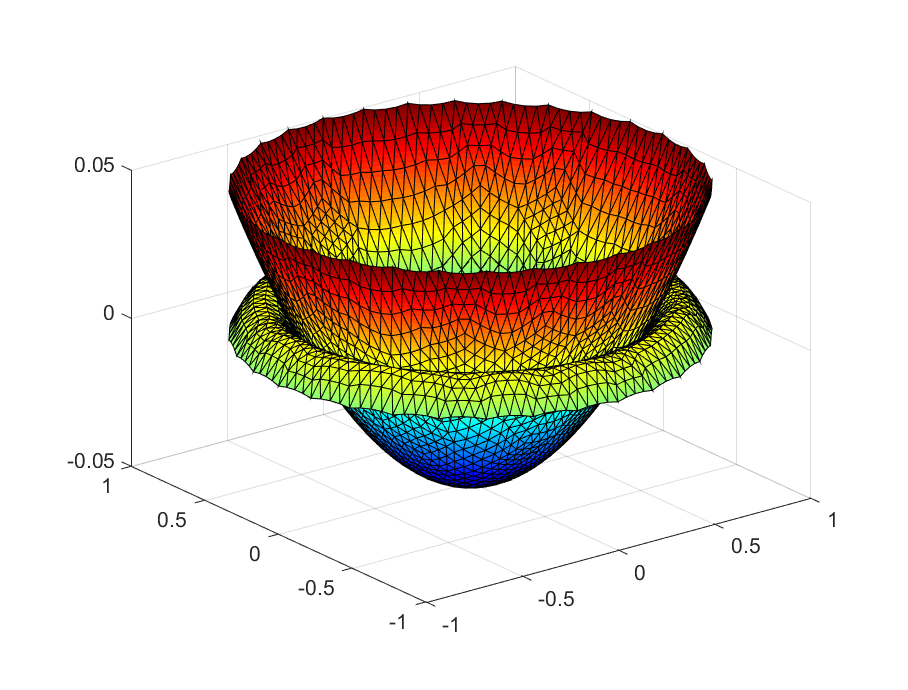
\includegraphics[width=\textwidth]{position_membrane_exact_resolution_convergence.eps}    
\label{ref:position_membrane_convergence}

\end{subfigure}
\begin{subfigure}[normal]{0.49\textwidth}
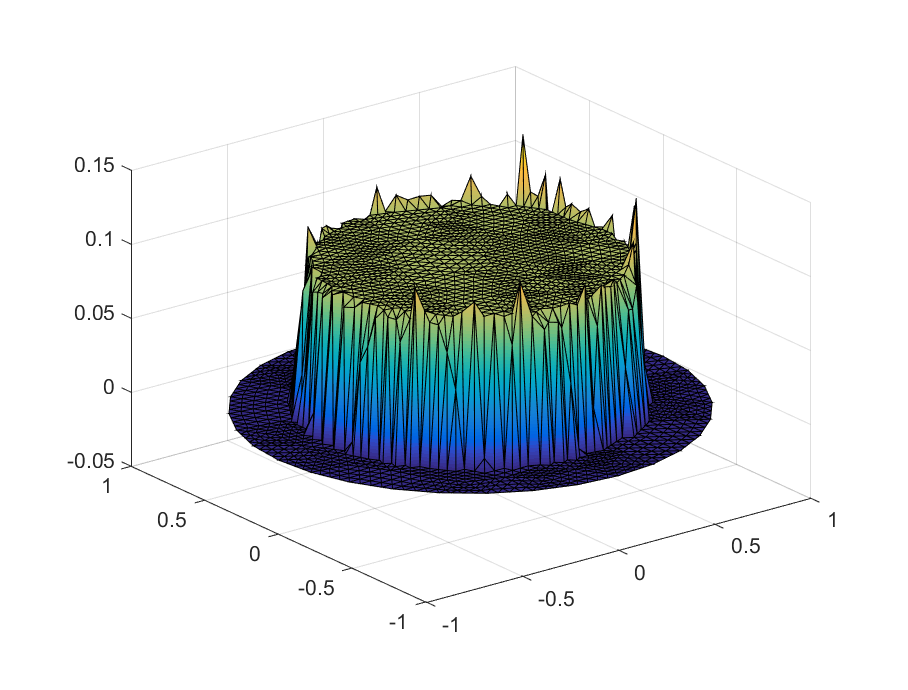
\includegraphics[width=\textwidth]{lambda_exact_resolution_convergence_J_3.eps}     
\label{ref:lambda_membrane_convergence} 
\end{subfigure}
\end{figure}
\vspace*{-4cm}\hspace*{0.75cm}$u_1$\\
\vspace*{0.6cm}\hspace*{0.75cm}$u_2$
\end{frame}
%\begin{frame}
%\frametitle{Introduction}
%\textbf{\textcolor{red}{Motivation}}
%\begin{itemize}
%\item
%Finite element discretization: 
%$\mathcal{A}(\Xh) = \bF$. 
%\item 
%Resolution via inexact \textbf{semi smooth} Newton method 
%%s$\mathbb{A}^{k-1}\Xhki + \Rhki = \bF^{\textcolor{blue}{k}-1}$
%\item
%A posteriori error estimate: 
%$\dps |||\bu-\uhki||| \leq \left\{\sum_{K \in\Th}\eta_K^2(\uhki)\right\}^{\frac{1}{2}}$.
%\item Adaptive inexact resolution and  adaptive stopping criteria.
%\item Numerical experiments to confirm the strength of our method.
%\end{itemize}
%\footnotesize
%\begin{thebibliography}{10}
%\bibitem{VorErn:2013}
%Alexandre Ern and Martin Vohral{\'{\i}}k.
%\newblock Adaptive inexact {N}ewton methods with a posteriori stopping criteria
%  for nonlinear diffusion {PDE}s. {\em SIAM J. Sci. Comput.}, 35(4):A1761--A1791, 2013.
%\end{thebibliography}
%\end{frame}
\begin{frame}
\section{Model problem and its dicretization}
\subsection{Model problem and its dicretization}  
\frametitle{Continuous model problem and setting}
\textbf{Notation}
\begin{itemize}
\item $H_g^1(\Omega)\hspace{-0.1 cm} =\hspace{-0.1 cm} \left\{u\in H^1(\Omega), \hspace{0.1 cm} u=g \hspace{0.1 cm} \mbox{on} \hspace{0.1 cm} \partial \Omega\right\}$
\item $\Lambda=\left\{\chi\in L^2(\Omega), \: \textcolor{carmine}{\chi \geq 0} \: \mbox{on} \hspace{0.1 cm} \Omega\right\}$
\item
$\mathcal{K}_g= \left\{(v_1,v_2)\in H_g^1(\Omega)\times H_0^1(\Omega),\: \textcolor{electricpurple}{v_1-v_2 \geq 0} \; \; \mbox{on} 
\hspace{0.1 cm} \Omega \right\}$
\end{itemize}
\textbf{Weak formulation:}
For $(f_1,f_2)\in L^2(\Omega)\times L^2 (\Omega)$ and $g > 0$ find $(u_1,u_2,\lambda)\in H_g^1(\Omega)\times H_0^1(\Omega) \times \Lambda$ such that
\begin{equation*}
\left\lbrace\begin{array}{llccc}
\dps \sum_{\ialf=1}^2 \mu_i \left(\nab u_i,\nab v_i\right)_{\Omega} - \left(\lambda,v_1-v_2\right)_{\Omega} = \sum_{\ialf=1}^2\left(f_i,v_i\right)_{\Omega} \quad \forall (v_1,v_2) \in H_0^1(\Omega)\times H_0^1(\Omega) \\
\left(\chi - \lambda,u_1-u_2\right)_{\Omega} \geq 0 
\quad \forall \chi \in \Lambda.
\end{array}
\right.
\label{eq:formulation_variationnelle_probleme_initial}
\end{equation*}
\textcolor{red}{\textbf{Existence and uniqueness: Lions-Stamppachia Theorem}}
\scriptsize
\begin{thebibliography}{10}
  \bibitem{VorBer:2008}
Faker Ben~Belgacem, Christine Bernardi, Adel Blouza, and Martin
  Vohral{\'{\i}}k.
\newblock A finite element discretization of the contact between two membranes.
\newblock {\em M2AN Math. Model. Numer. Anal.}, 43(1):33--52, 2008.
\end{thebibliography}
\end{frame}
\begin{frame}
\frametitle{Discretization by finite elements}
\textbf{Notation:} 
%Let $\Th$ be a conforming mesh of $\Omega$ in the sens of Ciarlet. 
\begin{itemize}
\item
$\Th$: conforming mesh, $\omega_\ba$: patch of elements of $\Th$ that share $\ba$
%\item 
%$\Vh$: vertices of $\Th$, $\Vhint$: interior vertices, $\Vhext$: exterior vertices. 
%\item 
%$\omega_\ba$: patch of elements of $\Th$ that share $\ba$ and ${\bf n}_{\omega_{h}^{\ba}}$ its outward unit normal.
%\item  
%$\psi_{h,\ba}$: Lagrange basis functions,
%$N_{h,\ba}$: Nnumber of elements forming a support of the basis functions
%\item
%$N_{h,\ba}$: Nnumber of elements forming a support of the basis functions, $\ba \in \Vhint$
%\item
%$h_K$: diameter of a triangle $K$.\quad $h=\max h_K$, $M_{\ba} = \left(\psi_{h,{\ba}},1\right)_{\omega_{\ba}} > 0$ 
\end{itemize}
\vspace{0.2 cm}
\textbf{Conforming spaces for the discretization:}
\begin{itemize}
%\item ${\mathbb{X}}_h=\left\{v_h \in \mathcal{C}^0(\overline{\Omega}), \forall K \in {\mathcal{T}}_h, {v_h}_{|K} \in {\mathbb{P}}_1 (K)\right\}$, 
\item
${\mathbb{X}}_{gh}=\left\{v_h \in \mathcal{C}^0(\overline{\Omega}), \forall K \in {\mathcal{T}}_h, {v_h}_{|K} \in {\mathbb{P}}_1 (K), \hspace{0.2 cm} v_h=g \hspace{0.2 cm} \mbox{on} \hspace{0.2 cm} \partial \Omega\right\}$
\item  
%${\mathbb{X}}_{0h}={\mathbb{X}}_h \cap H_0^1(\Omega)$, 
$\dps \Kgh=\left\{(v_{1h},v_{2h}) \in {\mathbb {X}}_{gh} \times {\mathbb{X}}_{0h}, \hspace{0.2 cm} \textcolor{electricpurple}{v_{1h}-v_{2h} \geq 0} \hspace{0.2 cm} \mbox{on} \hspace{0.2 cm} \Omega\right\}$
\item $\Lambda_h=\left\{\lambda_h \in \mathbb{X}_{0h}; \hspace{0.15 cm} \textcolor{carmine}{\lambda_h({\ba}) \geq 0} \quad \forall {\ba}\in \mathcal{V}_h^{\mathrm{int}}\right\}$.
\end{itemize}
\vspace{0.5 cm}
\textbf{Discretization:}
find $(u_{1h},u_{2h},\lambda_h)\in {\mathbb{X}}_{gh} \times {\mathbb{X}}_{0h} \times \Lambda_h$  such that $\forall (v_{1h},v_{2h}, \chi_h) \in {\mathbb{X}}_{0h} \times {\mathbb{X}}_{0h} \times \Lambda_h$
\begin{equation*}
\left\lbrace\begin{array}{llccc}
\dps \sum_{\ialf=1}^2 \mu_i \left(\nab u_{ih},\nab v_{ih}\right)_{\Omega} - \sum_{{\ba}\in \Vhint} \lambda_h({\ba})(v_{1h}-v_{2h})({\ba}) (\psi_{h,\ba}, 1)_{\oma}= \sum_{\ialf=1}^2 (f_i,v_{ih})_{\Omega}, \\
\textcolor{electricpurple}{(u_{1h}-u_{2h})(\ba) \geq 0}, \: \textcolor{carmine}{\lambda_h(\ba) \geq 0}, \: \textcolor{carmine}{\lambda_h(\ba)} \textcolor{electricpurple}{(u_{1h}-u_{2h})(\ba)}=0.
\end{array}
\right.
\end{equation*}
\end{frame}
\begin{frame}
\frametitle{Discrete complementarity problem}
\alert{\textbf{To reformulate the discrete constraints:}}
\begin{definition}
A function $f: {{\R}^n \times \R^n} \rightarrow \R^n$ is a C-function if
\begin{equation*}
\forall(\ba,\bb)\in {\R}^n \times \R^n \quad f(\ba,\bb)=0 \quad \iff \quad
\ba \geq0, \quad \bb \geq0, \quad \ba \bb=0.
\end{equation*}
\end{definition}
For any C-function ${\bf C}$, the discretization reads 
\begin{equation*}
\left\lbrace\begin{array}{llccc}
 \mathbb{E}\Xh &= \bF\\
{\bf C}(\X_h)&=0.
\end{array}
\right.
\quad \mbox{\textcolor{red}{\textbf{$\bf C$ is not Fréchet differentiable!}}}
\end{equation*}

%\begin{equation*}
%\left\lbrace\begin{array}{llccc}
% \mathbb{E}\Xh &= \bF\\
%{\bf C}(\X_h)&=0.
%\end{array}
%\right.
%\hspace{0.2 cm} \mbox{with} \hspace{0.2 cm} \mathbb{E}=
%\begin{pmatrix}
%\mu_1 \mathbb{A}_1 & {\Huge 0} & -{\Huge {\mathbb{D}}^{T}} \\
%{\Huge 0} &\mu_2 \mathbb{A}_1 &{\Huge {\mathbb{D}}^{T}} 
%\end{pmatrix}
%\hspace{0.2 cm} \mathbb{A}_1= \left(\nab \psi_{\ba_j},\nab \psi_{\ba_i}\right)_{1\leq i,j \leq N_h}
%%\label{eq:function:Pi}
%\end{equation*}
%where
%
%\begin{equation*}
% \mathbb{D} =\left(\psi_{\ba_i},1 \right)_{1 \leq i \leq  N_h} \quad
%\bF=
%\begin{pmatrix}
% \left(f_1 \psi_{h,{\ba}_l}-\mu_1\nab \tilde{g_h} \cdot \nab \psi_{h,{\ba}_l},1\right)_{\Omega}\\
%\left(f_2,\psi_{h,{\ba}_l}\right)_{\Omega}
%\end{pmatrix} \quad \forall 1 \leq l \leq N_h
%\end{equation*}
\textcolor{cadmiumgreen}{\textbf{ Example: semi-smooth "min" function}} 
\begin{equation*}
\CFun(\bXunh-\bXdeuxh,\bXtroish) =\min \left(\bXunh-\bXdeuxh, \bXtroish\right)
\end{equation*}
\textcolor{cadmiumgreen}{\textbf{Example: semi-smooth "Fischer-Burmeister" function}}
\begin{equation*}
\CFun(\bXunh-\bXdeuxh,\bXtroish)=\sqrt{\left(\bXunh-\bXdeuxh\right)^2 + \bXtroish^2} - (\bXunh-\bXdeuxh + \bXtroish)
\end{equation*}
The vector of unknowns has the following block structure
\begin{equation*}
\Xh^{T}=
%\left(\uunh(\ba_1) \cdots %\uunh(\ba_{N_h}),\udeuxh(\ba_1) \cdots %\udeuxh(\ba_{N_h}),{\lambda_h}(\ba_1) %\cdots {\lambda_h}(\ba_{N_h})\right)^{T}=
\left(\bXunh, \bXdeuxh, \bXtroish\right)^{T} \in \mathcal{M}_{3N_h,1}(\R)
%\label{eq:def:unknown:Xh}
\end{equation*}
\end{frame}
\section{Semi-smooth Newton method}
\subsection{Semi-smooth Newton method}
\begin{frame}
\frametitle{Semi-smooth Newton method}
For $\Xh^{0}$ given, the semi-smooth Newton method reads
\begin{equation*}
\mathbb{A}^{\textcolor{royalblue}{k-1}}\Xh^{\textcolor{royalblue}{k}}=\bB^{\textcolor{royalblue}{k-1}} \quad \forall \textcolor{royalblue}{k \geq 1}
%\label{eq:Newton_method}
\end{equation*}
The Clark Jacobian matrix and the right-hand side vector are defined by 
\begin{equation*}
\dps \mathbb{A}^{\textcolor{royalblue}{k-1}}=
\left\lbrace\begin{array}{llccc}
\mathbb{E}\\
{\bf J}_{\bf C}(\Xh^{\textcolor{royalblue}{k-1}})
\end{array}
\right.
\quad \mbox{and} \quad \bB^{\textcolor{royalblue}{k-1}} =
\left\lbrace\begin{array}{llccc}
\bF\\
{\bf J}_{\bf C}(\Xh^{\textcolor{royalblue}{k-1}})\Xh^{\textcolor{royalblue}{k-1}}-{\bf C}(\Xh^{\textcolor{royalblue}{k-1}})
\end{array}
\right.
\quad  \forall \textcolor{royalblue}{k\geq 1}.
\label{eq:def:jac_clarke:A:right:hand:side:newton:newton}
\end{equation*}
%Here, ${\bf J}_{\bf C}$ refers to the Clark Jacobian matrix of the semi-smooth function $\bC$. 

\textcolor{cadmiumgreen}{\textbf{ Example: Clark Jacobian matrix for the "min" function}} 

\begin{equation*}
\footnotesize
\mathbb{K} \! = \!
 \begin{pmatrix}
    1      & \cdots & 0 &-1      & \cdots & 0 & 0      & \cdots & 0  \\ 
    \vdots & \ddots & \vdots & \vdots & \ddots & \vdots & \vdots & \ddots & \vdots\\ 
    0      & \cdots & 1 & 0      & \cdots & -1 & 0      & \cdots & 0
\end{pmatrix}
 \hspace{0.02 cm}
\mathbb{G} \! = \!
\begin{pmatrix}
0      & \cdots & 0  &   0      & \cdots & 0 &1      & \cdots & 0  \\ 
    \vdots & \ddots & \vdots & \vdots & \ddots & \vdots & \vdots & \ddots & \vdots
    \\ 
0      & \cdots & 0  &  0      & \cdots & 0 & 0      & \cdots & 1 
\end{pmatrix},
%\label{eq: Jac_C_Kmat_G_mat}
\end{equation*}


\begin{equation*}
\JacCFun(\Xhk)_l
=
\begin{cases}
\mathbb{K}_l \quad \mbox{if} \quad \uunhk(\ba_l)-\udeuxhk(\ba_l) \leq \lambhk(\ba_l)\\
\mathbb{G}_l \quad \mbox{if} \quad \lambhk(\ba_l) < \uunhk(\ba_l)-\udeuxhk(\ba_l)
\end{cases}
\end{equation*}

\end{frame}
\begin{frame}
%\subsection{Algebraic resolution in semi-smooth Newton method}
\frametitle{Algebraic resolution in semi-smooth Newton method}
Any iterative algebraic
solver yields on step $i \geq 0$:
\begin{equation*}
\mathbb{A}^{\textcolor{royalblue}{k-1}}\Xhki + \Rhki=\bB^{\textcolor{royalblue}{k-1}}
%\label{eq:inexact_newton_method}
\end{equation*}
with $\Rhki=(\Runhki,\Rdeuxhki,\Rtroishki)^{T}$ the algebraic residual block vector.
%The vector of unknowns $\Xhki \in \mathcal{M}_{3N_h,1}(\R)$ is defined by 
%$(\Xhki)^{T} 
%%\left(\uunhki(\ba_1) \cdots \uunhki(\ba_{N_h}),\udeuxhki(\ba_1) \cdots \udeuxhki(\ba_{N_h}),{\lambda_h}^{k,i}(\ba_1) \cdots {\lambda_h}^{k,i}(\ba_{N_h})\right)^{T}
%=\left(\bXunhki, \bXdeuxhki, \bXtroishki\right)^{T}.$
\begin{definition}
We define discontinous $\mathbb{P}_1$ polynomials $\runhki$ and $\rdeuxhki$ %vanishing on the boundary of $\Omega$ satisfying
\begin{itemize}
\item $\dps (\runhki, \psi_{h,\ba_l})_K=\frac{(\Runhki)_l}{N_{h,\ba}}, \; {\runhki}_{|\partial K \cap \partial \Omega} =0 \qquad \forall 1 \leq l \leq N_h$
\item $\dps (\rdeuxhki, \psi_{h,\ba_l})_K=\frac{(\Rdeuxhki)_l}{N_{h,\ba}}, \; {\rdeuxhki}_{|\partial K \cap \partial \Omega} =0 \qquad \forall 1 \leq l \leq N_h$
\end{itemize}
\end{definition}

%
%for all basis functions $\psi_{h,\ba}$ of the space $\mathbb{X}_{0h}$.
%This leads naturally to the result
%\begin{equation}
%(\Runhki)_l=(\runhki,\psi_{h,\ba_l})_{\Omega} \quad \mbox{and} \quad (\Rdeuxhki)_l=(\rdeuxhki,\psi_{h,\ba_l})_{\Omega} \quad \forall l = 1 \cdots N_h.
%\label{eq:ecriture_variationnelle_résidu}
%\end{equation}
\textbf{Equivalent form of the $2N_h$ first equations}
%The $2N_h$ first lines of \eqref{eq:inexact_newton_method} reads
\begin{align*}
%\left\lbrace\begin{array}{rclrcl}
\nonumber\mu_1\dps \left(\nab \uunhki, \nab \psi_{h,{{\ba}_l}}\right)_{\Omega}&=\left(f_1+\lambhki({{\ba}_l})-\runhki,\psi_{h,\ba_l}\right)_{\Omega},\\
\mu_2 \dps \left(\nab \udeuxhki, \nab \psi_{h,{{\ba}_l}}\right)_{\Omega}&=    \left(f_2-\lambhki({{\ba}_l})-\rdeuxhki, \psi_{h,{\ba}_l}\right)_{\Omega}.
%\end{array}
%\right.
\label{eq:variational:formulation:inexacte_newton}
\end{align*}
\end{frame}

\begin{frame}
\section{A posteriori and adaptivity}
\subsection{A posteriori and adaptivity}
\frametitle{A posteriori analysis and preliminary study}
\alert{\textbf{A posteriori error estimates:}}
$\dps |||\bu-\uhki||| \leq \left\{\dps \sum_{\substack{K \in\Th}} \eta_K(\uhki)^2\right\}^{1/2}$.\\

%\alert{\textbf{Effectivity index:}} $\mathrm{I_{eff}}=\left\{\dps \sum_{\substack{K \in\Th}} \eta_K(\uhki)^2\right\}^{1/2} {\large /} \; {\dps|||\bu-\uhki|||} \quad \alert{\searrow 1} $ 
%From \eqref{eq:modele_initial_membrane} if we define ${\bm \sigma}_1 = -\mu_1 \nab u_1$ and ${\bm \sigma}_2 = - \mu_2 \nab u_2$ we have $({\bm \sigma}_1,{\bm \sigma}_2) \in \HdivOmeg$,  and $\nab \cdot {\bm \sigma}_1 = f_1 + \lambda $ and $\nab \cdot {\bm \sigma}_2 = f_2 - \lambda $. \\\\
%
\includegraphics[scale=0.02]{attention} 
%\footnotesize
%$\left(-\nab \uunhki, -\nab \udeuxhki\right) \neq \HdivOmeg \hspace{0.1 cm}$  $\nab \cdot (- \mu_1 \nab \uunhki) \neq f_1 + \lambhki$  $\nab \cdot (-\mu_2 \nab \udeuxhki) \neq f_2 - \lambhki$.
%\normalsize
\scriptsize{
\begin{thebibliography}{10}
\bibitem{Repin:2008}
Sergey Repin.
\newblock {\em A posteriori estimates for partial differential equations}.
\newblock Walter de Gruyter GmbH \& Co. KG, Berlin, 2008.
\end{thebibliography}
}

\scriptsize{
\begin{thebibliography}{10}
\bibitem{Verfurth:2013}
Verf\"urth, R\"udiger.
\newblock {\em A posteriori error estimation techniques for finite element
              methods}.
\newblock Oxford University Press, 2013.
\end{thebibliography}
}

\vspace{-0.3 cm}
\normalsize
\begin{equation*}
\mbox{\textbf{Goal:}}\dps
\left\lbrace\begin{array}{llccc}
\dps \sigunhki \in \textbf H(\div,\Omega) \hspace{0.15 cm} \mbox{such that} \hspace{0.15 cm} (\nab \cdot \sigunhki,1)_K=(f_1+\lambhki,1)_K \hspace{0.15 cm} \forall K \in \Th, \\
\dps\sigdeuxhki \in \textbf H(\div,\Omega) \hspace{0.15 cm} \mbox{such that} \hspace{0.15 cm} (\nab \cdot \sigdeuxhki,1)_K=(f_2-\lambhki,1)_K \hspace{0.15 cm} \forall K \in \Th .
\end{array}
\right.
%\label{eq: 1.24}
\end{equation*}
\normalsize
\begin{itemize}
\item 
$\sigunhki = \sigunhdiski + \sigunhalgki$ and $\sigdeuxhki = \sigdeuxhdiski + \sigdeuxhalgki$
\end{itemize}

%\textcolor{red}{\textbf{Assumption:}}
%$\sigunhalgki+\sigunhdiski =\sigunhki$ and
%$\sigdeuxhalgki+\sigdeuxhdiski =\sigdeuxhki$
%\\
\vspace{0.3 cm}
\textcolor{red}{\textbf{Algebraic fluxes reconstruction:}}
\begin{itemize}

%$\lim\limits_{\substack{\textcolor{blue}{k},\textcolor{red}{i} \rightarrow + \infty}} {\left\|\sigunhalgki\right\|}_{L^2(\Omega)} = \lim\limits_{\substack{\textcolor{blue}{k},\textcolor{red}{i} \rightarrow + \infty }} {\left\|\sigdeuxhalgki\right\|}_{L^2(\Omega)} = 0$
\item $\left\{\sigunhalgki,\sigdeuxhalgki\right\} \in \textbf H(\div,\Omega)$, \: $\nab \cdot \sigunhalgki=\runhki$, \: $\nab \cdot \sigdeuxhalgki=\rdeuxhki$
\end{itemize}



\scriptsize
\begin{thebibliography}{10}
  \bibitem{VorPapez:2015}
Papez Jan, Rüde Ulrich, Vohral{\'{\i}}k Martin, and Wohlmuth Barbara.
\newblock Sharp algebraic and total a posteriori error bounds via a multilevel
approach.
\newblock In preparation, 2017.
\end{thebibliography}
\end{frame}
%\subsection{Discretization fluxes reconstruction}
\begin{frame}
\frametitle{Discretization fluxes reconstruction}
%\subsection{Discretization flux reconstruction}
%$\forall \ba \in \mathcal{V}_{h}$, define $(\sigunhdiskia,\sigdeuxhdiskia) \in {\bf V}_{h}^{\ba} \times {\bf V}_{h}^{\ba}$ and $(\gamunhkia,\gamdeuxhkia)\in Q_{h}^{\ba} \times Q_{h}^{\ba}$, where ${\bf V}_{h}^{\ba} \subset \textbf H(\div,\Omega)$ and $Q_{h}^{\ba} \subset L^2(\Omega)$ by solving:
$\sigunhdiskia$ and $\sigdeuxhdiskia$ are the solution of mixed system on patches
\begin{equation*}
\left\lbrace\begin{array}{llccc}
(\sigunhdiskia,{\bv}_{1h})_{\omega_{h}^{\ba}}-(\gamunhkia,\nab \cdot {\bv}_{1h})_{\omega_{h}^{\ba}} &=& \dps -\left(\psi_{h,\ba} \nab \uunhki,{\bv}_{1h}\right)_{\omega_h^{\ba}}  & \forall {\bv}_{1h}\in {\bf V}_{h}^{\ba}, \\
\dps(\nab \cdot \sigunhdiskia,q_{1h})_{\omega_{h}^{\ba}}&=&\dps(\tildgunhkia,q_{1h})_{\omega_{h}^{\ba}} & \forall q_{1h}\in Q_{h}^{\ba},\\
(\sigdeuxhdiskia,{\bv}_{2h})_{\omega_{h}^{\ba}}-(\gamdeuxhkia,\nab \cdot {\bv}_{2h})_{\omega_{h}^{\ba}} &=& \dps-\left(\psi_{h,\ba} \nab \udeuxhki,{\bv}_{2h}\right)_{\omega_h^{\ba}} & \forall {\bv}_{2h}\in {\bf V}_{h}^{\ba},\\
(\nab \cdot \sigdeuxhdiskia,q_{2h})_{\omega_{h}^{\ba}}&=&\dps(\tildgdeuxhkia,q_{2h})_{\omega_{h}^{\ba}} & \forall q_{2h} \in Q_{h}^{\ba}.
\end{array}
\right.
%\label{eq:reconstruction_flux_raviart_thomas:newton:min:inexacte:discretozation:flux}
\end{equation*}
%\begin{align*}
%\tildgunhkia &=f_1 \psi_{h,\ba}- \mu_1 \nab \uunhki \cdot \nab \psi_{h,\ba} +\lambhki(\ba)\psi_{h,\ba} -\runhki \psi_{h,\ba} \quad \forall {\ba} \in \mathcal{V}_{h},\\
%\tildgdeuxhkia &= f_2 \psi_{h,\ba}- \mu_2 \nab \udeuxhki \cdot \nab \psi_{h,\ba}-\lambhki(\ba)\psi_{h,\ba}-\rdeuxhki \psi_{h,\ba} \quad \forall {\ba} \in \mathcal{V}_h,
%\end{align*}
\hspace{1.2 cm}
\fcolorbox{violet}{white}{
\textcolor{black}{$\dps
{{\sigunhdiski}}={\sum_{\ba \in \mathcal{V}_h} \sigunhdiskia} \quad \mbox{and} \quad \sigdeuxhdiski=\sum_{\ba \in \mathcal{V}_h} \sigdeuxhdiskia$}
}
\begin{itemize}
\item
$\sigunhdiski  \in \textbf H(\div,\Omega) \quad \mbox{and} \quad \left(\nab \cdot \sigunhdiski, 1\right)_K = \left(f_1 + \lambhki -\runhki ,1\right)_K$
\item
$\sigdeuxhdiski \in \textbf H(\div,\Omega) \quad \mbox{and} \quad \left(\nab \cdot \sigdeuxhdiski, 1\right)_K = \left(f_2 - \lambhki -\rdeuxhki ,1\right)_K$ .
\end{itemize}


\scriptsize{
\begin{thebibliography}{10}
\bibitem{Braess:2009}
Braess, Dietrich and Pillwein, Veronika and Sch{\"o}berl,
              Joachim.
\newblock {\em Equilibrated residual error estimates are {$p$}-robust}.
\newblock Computer Methods in Applied Mechanics and Engineering, 2009.
\end{thebibliography}
}

\end{frame}
%\subsection{A posteriori error estimates}
\begin{frame}
\frametitle{A posteriori error estimates}
\vspace{-0.2 cm}

\begin{itemize}
\item
${\bm u}=(u_1,u_2)\in\mathcal{K}_g$,\ $\uhki=(\uunhki,\udeuxhki)\in \mathbb{X}_{gh} \times \mathbb{X}_{0h}$,\ $\left\{\sigunhki, \sigdeuxhki\right\} \in \HdivOmeg$
\end{itemize}
\textcolor{red}{\textbf{Warning:}}
$\uunhki(\ba) - \udeuxhki(\ba)$ and $\lambhki(\ba)$ can be negative. 
%\vspace{-0.3 cm}
\begin{figure}[H]
\textcolor{red}{\hspace{-1.4 cm} \textbf{Example: k=2}}
\begin{subfigure}[normal]{0.35\textwidth} 
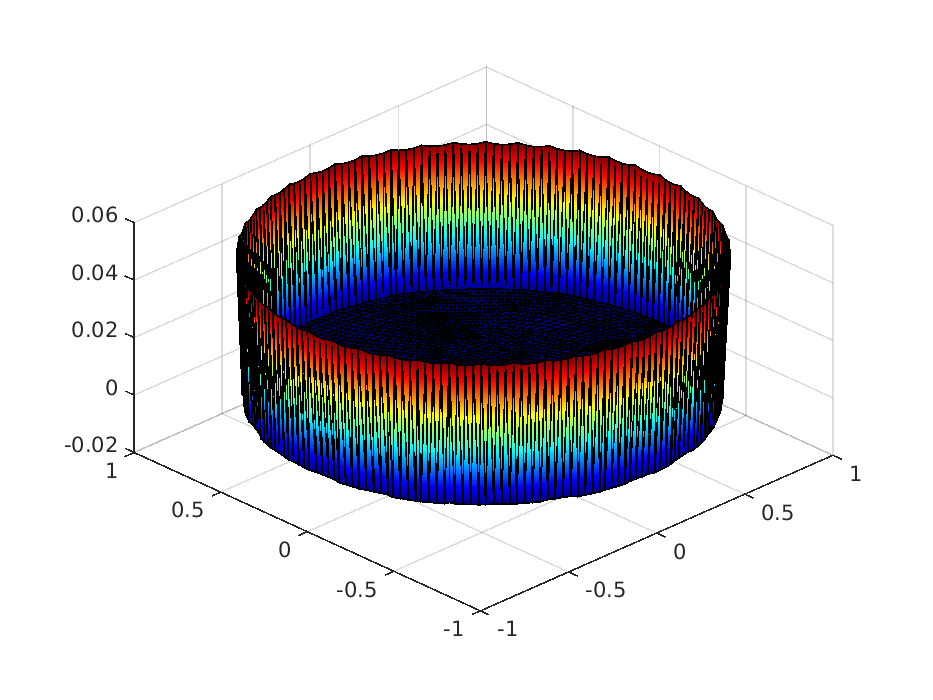
\includegraphics[width=\textwidth]{fig_article/diff_u1_u2_newton_gmres.eps}    
\label{ref:position_membrane_inside_iter}
\end{subfigure}
\begin{subfigure}[normal]{0.35\textwidth}
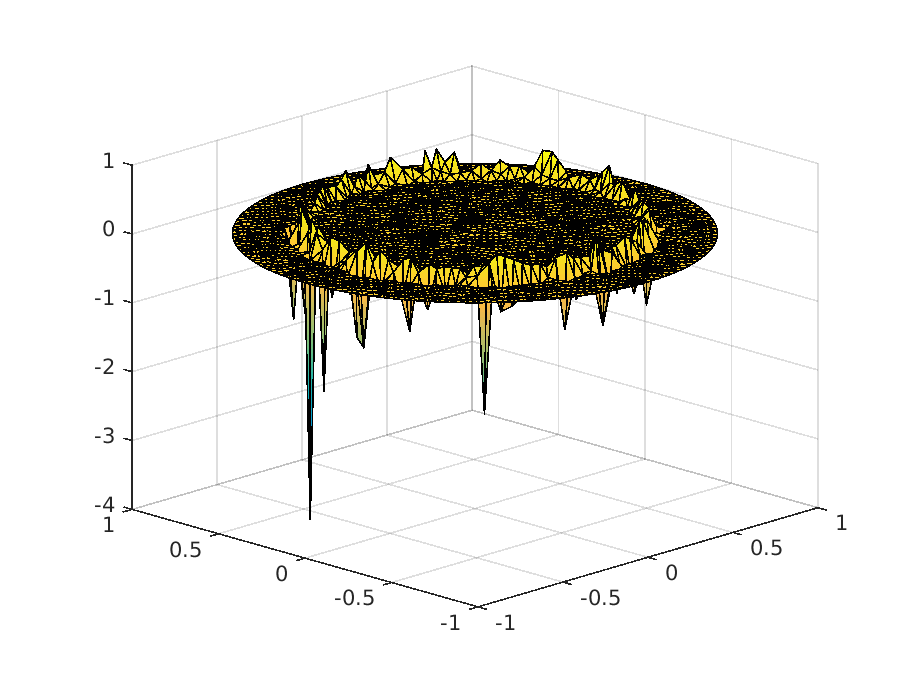
\includegraphics[width=\textwidth]{fig_article/lambda_newton_iter7.eps}     
\label{ref:lambda_membrane_inside_iter} 
\end{subfigure}
%\caption{membranes (left) and lagrange multiplier (right) during the iterations }
\end{figure}
\vspace{-0.2 cm}
\textcolor{cadmiumgreen}{\textbf{Motivation:}} Define $\shki \in \Kgh$ by
\vspace{0.3 cm}
$\dps \shki (\ba)= \dps \begin{cases}
\uhki(\ba) = \left(\uunhki(\ba), \udeuxhki(\ba)\right) \quad &\mbox{if $\uunhki(\ba) \geq \udeuxhki(\ba)$,}\\
\dps \left(\frac{\uunhki(\ba) + \udeuxhki(\ba)}{2}, \frac{\uunhki(\ba) + \udeuxhki(\ba)}{2}\right) \quad &\mbox{if $\uunhki(\ba) < \udeuxhki(\ba)$.}\end{cases}$
\end{frame}
\begin{frame}


\begin{itemize}
\item
Discretization error estimators
\vspace{0.3 cm}
$\left.
\begin{array}{ll}
\dps {\eta}_{\mathrm{F},K,\ialf}^{\textcolor{royalblue}{k},\textcolor{burntorange}{i}} &= \left\| \mu_\ialf^{\frac{1}{2}} \nab u_{\ialf h}^{\textcolor{royalblue}{k},\textcolor{burntorange}{i}}+\mu_\ialf^{-\frac{1}{2}} \sigmaialfhdiscki \right\|_{K}  
\\
\dps {\eta}_{\mathrm{osc},K,\ialf} & =  \dps \frac{h_K}{\pi} \mu_\ialf^{-\frac{1}{2}} \left\|f_\ialf-{\bm \Pi}_{\mathbb{P}_1}(f_\ialf)\right\|_{K}\\
\dps \etCKkipos & = 2 \dps \left(\uunhki-\udeuxhki,\lambhkipos\right)_K
\end{array}
\right\} \Rightarrow \dps {\bm \eta}^{\textcolor{royalblue}{k},\textcolor{burntorange}{i}}_{\mathrm{disc}}
$\\
%\vspace{0.2 cm}
\item
Linearization error estimators
\vspace{0.3 cm}
%%%%%%%%%%
$\left.
\begin{array}{ll}
\dps \etalinunKki  &=  \tnorm{\shki-\uhki}_K  
\\
\dps \etalindeuxKki &= 2 h_{\Omega} \CPF \left(\frac{1}{\mu_1} + \frac{1}{\mu_2} \right)^{\frac{1}{2}} \left\|\lambhkipos\right\|_{\Omega} \tnorm{\shki-\uhki}_K\\
\dps \etalintroisKki &= h_{\Omega} \CPF \left(\frac{1}{\mu_1} + \frac{1}{\mu_2} \right)^{\frac{1}{2}} \left\| \lambhkineg\right\|_K
\end{array}
\right\} \Rightarrow \dps {\bm \eta}^{\textcolor{royalblue}{k},\textcolor{burntorange}{i}}_{\mathrm{lin}}
$
\\
\item
Algebraic error estimators\\
\vspace{0.1 cm}
$\left.
\begin{array}{ll}
\dps \etaalgKialfki &= \left\|\mu_\ialf^{-\frac{1}{2}}\sigmaialfhalgki\right\|_{K}
\end{array}
\right\} \Rightarrow \dps {\bm \eta}^{\textcolor{royalblue}{k},\textcolor{burntorange}{i}}_{\mathrm{alg}}
$
\end{itemize}

\begin{theorem}[A posteriori  estimate distinguishing the error components]


\emph{
\textcolor{bulgarianrose}{
\begin{equation*}
\dps
|||\bu-\uhki||| \leq \eta^{\textcolor{royalblue}{k},\textcolor{burntorange}{i}}_{\mathrm{disc}} +\eta^{\textcolor{royalblue}{k},\textcolor{burntorange}{i}}_{\mathrm{alg}} + \eta^{\textcolor{royalblue}{k},\textcolor{burntorange}{i}}_{\mathrm{lin}}.
\end{equation*}
}}

\end{theorem}
\end{frame}

\begin{frame}
\vspace{-0.2 cm}
\begin{proof}
We define global versions of these estimators as $ \eta_{\cdot}^{k,i} = \left\{\sum_{K \in \Th}\left(\eta_{\cdot,K}^{k,i}\right)^2\right\}^{\frac{1}{2}}$
\begin{enumerate}
\item $\uhki \notin \Kgh$: define the projection 
$\bs$ of $\uhki$ in $\Kg$ by $a(\bs,\bv-\bs) \geq a(\uhki,\bv-\bs) \quad \forall \bv \in \Kg $ \alert{Pb well posed: Lions-Stampacchia}


\item<2-> 

$
\tnorm{\bu-\uhki}^2 = \underbrace{ a(\bu - \uhki, \bu - \bs)}_{=\textcolor{blue}{\textbf{A}}} + \underbrace{a(\bu  - \uhki, \bs-\uhki)}_{=\textcolor{cadmiumgreen}{\textbf{B}}}.
%=a(\bu,\bu-\uhki)-a(\uhki,\bu-\uhki).
$
\item<3-> 

$\textcolor{cadmiumgreen}{\textbf{B}} \leq \tnorm{\bu-\uhki} \etalinunki$
\item<4-> 
\footnotesize
\vspace{-0.3 cm}
$\dps
\textcolor{blue}{\textbf{A}} \leq \left(\underbrace{\left\{\dps \sum_{K \in \Th}\dps \sum_{\ialf=1}^2({\eta}_{\mathrm{osc},K,\ialf} + {\eta}_{\mathrm{F},K,\ialf}^{\textcolor{royalblue}{k},\textcolor{burntorange}{i}})^2\right\}^{\frac{1}{2}}}_{\textcolor{bulgarianrose}{\eta_1}} + \etalintroiski \right) \tnorm{\bu-\uhki} + \frac{1}{2} \etalindeuxki + \frac{1}{2} \sum_{K \in \Th} \etCKkipos 
$
\item<5-> 
\alert{Young inequality:} $\dps \tnorm{\bu-\uhki} \leq  \left\{ \left(\eta_1^{\textcolor{royalblue}{k},\textcolor{burntorange}{i}} + \etalinunki + \etalintroiski    \right)^2  + \etalindeuxki + \sum_K \etCKkipos \right\}^{\frac{1}{2}}.
$
\end{enumerate}
\end{proof}
\end{frame}

%\begin{frame}
%\scriptsize
%$\dps \eta_1 \hspace{-0.1 cm} = \left\{\sum_{K \in \Th}\sum_{j=1}^2({\eta}_{\mathrm{R},K,j}^{k,i}+{\eta}_{\mathrm{F},K,j}^{k,i}+\etalgKjki)^2\right\}^{\frac{1}{2}}$ $\dps \eta_2 \hspace{-0.1 cm}= \left\{\sum_{K\in \Th} (\etLKkineg)^2\right\}^{\frac{1}{2}} \hspace{-0.2 cm} +\left\{\sum_{K\in \Th} (\etPKki)^2\right\}^{\frac{1}{2}}$
%\\
%\scriptsize
%$\dps \eta_3 = \frac{1}{2} \sum_{K\in \Th}\left(\etCKkineg + \etCKkipos \right)+\left\{\sum_{K\in \Th} (\etLKkipos)^2\right\}^{\frac{1}{2}}$ 
%$\dps \varepsilon_1 = \frac{1}{2} \hspace{-0.1 cm} + \frac{1}{2}\frac{\min(1, \eta_2)}{\eta_2}$  $\dps \varepsilon_2 \hspace{-0.1 cm}=\min(\frac{1}{2}, \eta_2)$
%\vspace{-0.2 cm}
%\normalsize

%\begin{itemize}
%\item 
%$\dps \eta^{k,i}_{\mathrm{disc}} = \sqrt{2} \left\{3 \sum_{j=1}^{2}\left(\sum_{K \in \Th} \left({\eta}_{\mathrm{R},K,j}^{k,i} + {\eta}_{\mathrm{F},K,j}^{k,i}\right)^{2}\right) + \frac{1}{2} \sum_{K \in \Th} \etCKkipos \right\}^{\frac{1}{2}}$
%\item
%$\dps \eta^{k,i}_{\mathrm{alg}} =  \sqrt{6} \left\{\sum_{j=1}^{2} \sum_{K \in \Th} \left(\etalgKjki\right)^{2}\right\}^{\frac{1}{2}}$
%\item
%$\dps \eta^{k,i}_{\mathrm{lin}} = \sqrt{2} \left\{\sum_{K \in \Th} \left(2 \left(\etLKkineg + \etPKki\right)^2 + \frac{1}{2} \etCKkineg + \etLKkipos\right)\right\}^{\frac{1}{2}}$
%\end{itemize}

%\end{frame}
%\section{Adaptive Inexacte semi-smooth Newton method}

%%%%%%%%%%%%%%%%%%%%%%ADAPTIVE ALGORITHM IF FOR
%\begin{frame}
%\frametitle{Adaptive inexacte semi-smooth Newton algorithm}
%%\vspace{-0.3 cm}
%\vspace{-0.4 cm}
%\begin{algorithm}[H]
%\caption{Adaptive inexact semi-smooth Newton algorithm}
%
%\begin{algorithmic}
%\STATE{\textbf{Initialization:}\; Choose an initial vector $\Xh^{\textcolor{royalblue}{0}} \in \mathcal{M}_{3N_h,1}(\R)$}
%\FOR{$\textcolor{royalblue}{k=1 : N_{\mathrm{newton}}^{\mathrm{max}}}$} 
%\STATE {Compute $\A^{\textcolor{royalblue}{k-1}} \hspace{-0.1
% cm} \in \mathcal{M}_{3N_h,3N_h}(\R)$, $\bB^{\textcolor{royalblue}{k-1}} \hspace{-0.1 cm} \in \mathcal{M}_{3N_h,1}(\R)$ \\
%Consider 
%%the system of linear algebraic equations 
%$\A^{\textcolor{royalblue}{k-1}} \Xhk= \bB^{\textcolor{royalblue}{k-1}}$}
%\STATE{\textbf{Initialization for the linear solver:} Define $\X_h^{\textcolor{royalblue}{k},\textcolor{burntorange}{0}} = \X_h^{\textcolor{royalblue}{k-1}}$ 
%%as initial guess for the linear solver 
%}
%	\FOR{$\textcolor{burntorange}{i=1 : N_{\mathrm{alg}}^{\mathrm{max}}}$}\STATE Compute Residual: {$\Rhki =\bB^{\textcolor{royalblue}{k-1}}-\A^{\textcolor{royalblue}{k-1}} \Xhki$}\\
%	Compute estimators 
%	\IF{\fcolorbox{violet}{white}{$\eta_{\mathrm{alg}}^{\textcolor{royalblue}{k},\textcolor{burntorange}{i}} \leq \gamma_{\mathrm{alg}} \max  \left\{{\eta_{\mathrm{disc}}^{\textcolor{royalblue}{k},\textcolor{burntorange}{i}}, \eta_{\mathrm{lin}}^{\textcolor{royalblue}{k},\textcolor{burntorange}{i}}}\right\}$}} \STATE {Set $\Xhk = \Xhki$ end of linear solver (\textbf{break})} 
%	%\ELSE \STATE{$\textcolor{burntorange}{i}=\textcolor{burntorange}{i}+1$}
%	\ENDIF
%	\ENDFOR
%	\IF{\fcolorbox{violet}{white}{$\eta_{\mathrm{lin}}^{\textcolor{royalblue}{k},\textcolor{burntorange}{i}} \leq \gamma_{\mathrm{lin}} \eta_{\mathrm{disc}}^{\textcolor{royalblue}{k},\textcolor{burntorange}{i}}$}} \STATE {Set $\Xhk = \Xh$, end of non linear solver (\textbf{return})} 
%%	\ELSE \STATE{$\textcolor{royalblue}{k}=\textcolor{royalblue}{k}+1$} 
%\ENDIF
%\ENDFOR
%\end{algorithmic}
%\end{algorithm}
%\scriptsize
%\vspace{-0.4 cm}
%%\begin{thebibliography}{10}
%%\bibitem{VorErn:2013}
%%Alexandre Ern and Martin Vohral{\'{\i}}k.
%%\newblock Adaptive inexact {N}ewton methods with a posteriori stopping criteria
%%  for nonlinear diffusion {PDE}s. {\em SIAM J. Sci. Comput.}, 35(4):A1761--A1791, 2013.
%%\end{thebibliography}
%\end{frame}
%\begin{frame}
%\scriptsize
%\vspace{-0.3 cm}
%\begin{algorithm}[H]
%\caption{Adaptive Inexact semi-smooth Newton algorithm}
%\begin{algorithmic}
%\STATE $ {\bm 1.} \hspace{0.1 cm} \mbox{Choose an initial vector $\Xh^{0} \in \mathcal{M}_{3N_h,1}(\R)$ \hspace{0.15 cm} and we set $\textcolor{royalblue}{k}=1$}.$\\
%\vspace{0.1 cm}
%\STATE $ {\bm 2.} \hspace{0.1 cm} \mbox{From $\Xh^{k-1}$ define $\A^{\textcolor{royalblue}{k}-1} \in \mathcal{M}_{3N_h,3N_h}(\R)$ and $\mathbb{F}^{\textcolor{royalblue}{k}-1} \in \mathcal{M}_{3N_h,1}(\R)$.}$\\
%\vspace{0.1 cm}
%\STATE  $ {\bm 3.}\hspace{0.1 cm} \mbox{Consider the system of linear algebraic equations $\A^{\textcolor{royalblue}{k}-1} \Xhk= \mathbb{F}^{\textcolor{royalblue}{k}-1}$ ($*$)}$.\\
%\vspace{0.1 cm}
%\STATE  ${\bm {3a}.} \hspace{0.1 cm} \mbox{Define $\X_h^{\textcolor{royalblue}{k},0} = \X_h^{k-1}$ as initial guess for the linear solver and set $\textcolor{burntorange}{i}=0$}$.\\
%\vspace{0.1 cm}
%\STATE  ${\bm {3b}.}\hspace{0.1 cm}  \mbox{For $\textcolor{red}{\textcolor{burntorange}{i}}>0$ the approximation $\Xhki$ to $\Xhk$ satisfy $\A^{\textcolor{royalblue}{k}-1} \Xhki +\Rhki =\mathbb{F}^{\textcolor{royalblue}{k}-1}$ ($**$)}$.\\
%\vspace{0.1 cm}
%\STATE ${\bm 4.}\hspace{0.1 cm} \mbox{\textcolor{cadmiumgreen}{\textbf{Adaptive inexact resolution for ($**$)}}}$.\\
%\vspace{0.1 cm}
%\STATE $\qquad {\bm {4a}.} \hspace{0.1 cm} \mbox{Stopping criterion for the linear solver: $\eta_{\mathrm{alg}}^{\textcolor{royalblue}{k},\textcolor{burntorange}{i}} \leq \gamma_{\mathrm{alg}} \max \left\{\eta_{\mathrm{disc}}^{\textcolor{royalblue}{k},\textcolor{burntorange}{i}}, \eta_{\mathrm{lin}}^{\textcolor{royalblue}{k},\textcolor{burntorange}{i}}\right\}$.}$
%\vspace{0.1 cm}
%\STATE $ \qquad \mbox{If satisfied, set $\Xhk = \Xhki$. If not, set $\textcolor{burntorange}{i}=\textcolor{burntorange}{i}+1$ and go back to $(**)$.}$\\
%\vspace{0.1 cm}
%\STATE $\qquad {\bm {4b}.}\hspace{0.1 cm}  \mbox{Sopping criterion for the non linear solver: $\eta_{\mathrm{lin}}^{\textcolor{royalblue}{k},\textcolor{burntorange}{i}} \leq \gamma_{\mathrm{lin}} \eta_{\mathrm{disc}}^{\textcolor{royalblue}{k},\textcolor{burntorange}{i}}$.}$\\
%\vspace{0.1 cm}
%\STATE $\qquad \mbox{If satisfied finish. If not, set $\textcolor{royalblue}{k}=\textcolor{royalblue}{k}+1$ and go back to ${\bm 2}.$}$
%\label{ref:adpative:exact:inexacte algorithm}
%\end{algorithmic}
%\label{ref:methode_newton_min_exacte}
%\end{algorithm}
%\scriptsize
%\begin{thebibliography}{10}
%\bibitem{VorErn:2013}
%Alexandre Ern and Martin Vohral{\'{\i}}k.
%\newblock Adaptive inexact {N}ewton methods with a posteriori stopping criteria
%  for nonlinear diffusion {PDE}s. {\em SIAM J. Sci. Comput.}, 35(4):A1761--A1791, 2013.
%\end{thebibliography}
%\end{frame}

%%%%%%%%%ALGO LIKE PAPER MARTIN SIAM
%%%%%%%%%%%%%%
%\scriptsize
%\begin{algorithmic}
%\STATE $ {\bm 1.} \hspace{0.1 cm} \mbox{Choose an initial vector $\Xh^{0} \in \mathcal{M}_{3N_h,1}(\R)$ \hspace{0.15 cm} and we set $k=1$}.$\\
%\STATE $ {\bm 2.} \hspace{0.1 cm} \mbox{From $\Xh^{k-1}$ define the matrix $\A^{k-1} \in \mathcal{M}_{3N_h,3N_h}(\R)$ and the vector $\mathbb{F}^{k-1} \in \mathcal{M}_{3N_h,1}(\R)$  by \eqref{eq:def:jac_clarke:A:right:hand:side:newton:newton}.}$\\
%\STATE  $ {\bm 3.}\hspace{0.1 cm} \mbox{Consider the system of linear algebraic equations $\A^{k-1} \Xhk= \mathbb{F}^{k-1}$ ($*$)}$.\\
%\STATE  ${\bm {3a}.} \hspace{0.1 cm} \mbox{Define $\X_h^{k,0} = \X_h^{k-1}$ as initial guess for the iterative linear solver and set $i=0$}$.\\
%\STATE  ${\bm {3b}.}\hspace{0.1 cm}  \mbox{Perform $\nu$ steps of a chosen iterative lienar solver for the solution of the linear system $(*)$ starting}$\\
%\STATE $\mbox{from the vector $\Xhki$. This yields on step $i \geq 0$ an approximation $\Xhki$ to $\Xhk$ satisfying}$\\
%\STATE$\mbox{$\A^{k-1} \Xhki +\Rhki =\mathbb{F}^{k-1}$ ($**$)}$.\\
%\STATE ${\bm 4.}\hspace{0.1 cm} \mbox{\textcolor{blue}{Exact resolution for ($**$)}}$.\\
%\only<2>{
%\STATE $\qquad {\bm {4a}.}\hspace{0.1 cm}  \mbox{Check the stopping criterion for the linear solver in the form $\left\|\bR_{\mathrm{alg}} \right\| \leq \varepsilon_1$}$.\\
%\STATE $ \qquad\mbox{If satisfied, set $\Xhk = \Xhki$. If not, set $i=i+\nu$ and go back to ${\bm 3b}$.}$\\
%\STATE $\qquad {\bm {4b}.}\hspace{0.1 cm}  \mbox{Check the stopping criterion for the non linear solver in the form $\left\|\bR_{\mathrm{lin}} \right\| \leq \varepsilon_1$}$.\\
%\STATE $ \qquad\mbox{If satisfied finish. If not, set $k=k+1$ and go back to ${\bm 2}.$}$\\}
%\STATE ${\bm 5.}\hspace{0.1 cm} \mbox{\textcolor{cadmiumgreen}{Inexact resolution for ($**$)}}$.\\
%\only<3>{\STATE $\qquad {\bm {5a}.}\hspace{0.1 cm} \mbox{Check the stopping criterion for the linear solver in the form $\left\|\bR_{\mathrm{alg}} \right\| \leq \alpha_{\mathrm{alg}}\left\|\bR_{\mathrm{lin}} \right\|$}$.\\
%\STATE $ \qquad\mbox{If satisfied, set $\Xhk = \Xhki$. If not, set $i=i+\nu$ and go back to ${\bm {3b}}$}$.\\
%\STATE $\qquad {\bm {5b}.} \hspace{0.1 cm} \mbox{Check the stopping criterion for the non linear solver in the form $\left\|\bR_{\mathrm{lin}} \right\| \leq \varepsilon_1$}$.\\
%\STATE $ \qquad\mbox{If satisfied finish. If not, set $k=k+1$ and go back to ${\bm 2}.$}$\\
%}
%\STATE ${\bm 6.}\hspace{0.1 cm} \mbox{\textcolor{red}{Adaptive inexact resolution for ($**$)}}$.\\
%\only<4>
%{
%\STATE $\qquad {\bm {6a}.} \hspace{0.1 cm} \mbox{Check the stopping criterion for the linear solver in the form $\eta_{\mathrm{alg}}^{k,i} \leq \gamma_{\mathrm{alg}} \max \left\{\eta_{\mathrm{disc}}^{k,i}, \eta_{\mathrm{lin}}^{k,i}\right\}$.}$
%\STATE $ \qquad \mbox{If satisfied, set $\Xhk = \Xhki$. If not, set $i=i+1$ and go back to $(**)$.}$\\
%\STATE $\qquad {\bm {6b}.}\hspace{0.1 cm}  \mbox{Check the stopping criterion for the non linear solver in the form $\eta_{\mathrm{lin}}^{k,i} \leq \gamma_{\mathrm{lin}} \eta_{\mathrm{disc}}^{k,i}$.}$\\
%\STATE $\qquad \mbox{If satisfied finish. If not, set $k=k+1$ and go back to ${\bm 2}.$}$
%}
%\label{ref:adpative:exact:inexacte algorithm}
%\end{algorithmic}
%\label{ref:methode_newton_min_exacte}
%\end{algorithm}
%\end{frame}

\begin{frame}
\vspace{-0.3 cm}
\begin{algorithm}[H]
\frametitle{Adaptive inexacte semi-smooth Newton algorithm}
\caption{Adaptive inexact semi-smooth Newton algorithm}
\begin{algorithmic}

\STATE{\textbf{Initialization:}\; Choose an initial vector $\Xh^{\textcolor{royalblue}{0}} \in \mathcal{M}_{3N_h,1}(\R)$, ($\textcolor{royalblue}{k}=0$)}\\
\STATE{\textbf{Do}}\\
\STATE{\quad$\textcolor{royalblue}{k} =\textcolor{royalblue}{k+1}$}\\
\STATE {\quad Compute $\A^{\textcolor{royalblue}{k-1}} \hspace{-0.1
 cm} \in \mathcal{M}_{3N_h,3N_h}(\R)$, $\bB^{\textcolor{royalblue}{k-1}} \hspace{-0.1 cm} \in \mathcal{M}_{3N_h,1}(\R)$ \\
\quad Consider 
%the system of linear algebraic equations 
$\A^{\textcolor{royalblue}{k-1}} \Xhk= \bB^{\textcolor{royalblue}{k-1}}$}
\STATE{\quad \textbf{Initialization for the linear solver:} Define $\X_h^{\textcolor{royalblue}{k},\textcolor{burntorange}{0}} = \X_h^{\textcolor{royalblue}{k-1}}$, ($\textcolor{burntorange}{i=0}$) 
%as initial guess for the linear solver 
}\\
\STATE{\quad \textbf{Do}}
	\STATE{\qquad $\textcolor{burntorange}{i=i+1}$}\\	
	\STATE \qquad Compute Residual: {$\Rhki =\bB^{\textcolor{royalblue}{k-1}}-\A^{\textcolor{royalblue}{k-1}} \Xhki$}\\
	\qquad  Compute estimators 
	\STATE{\quad \textbf{While} \fcolorbox{violet}{white}{$\eta_{\mathrm{alg}}^{\textcolor{royalblue}{k},\textcolor{burntorange}{i}} \geq \gamma_{\mathrm{alg}} \max  \left\{{\eta_{\mathrm{disc}}^{\textcolor{royalblue}{k},\textcolor{burntorange}{i}}, \eta_{\mathrm{lin}}^{\textcolor{royalblue}{k},\textcolor{burntorange}{i}}}\right\}$}} 
	
	
	
	\STATE{\textbf{While} \fcolorbox{violet}{white}{ $\eta_{\mathrm{lin}}^{\textcolor{royalblue}{k},\textcolor{burntorange}{i}} \geq \gamma_{\mathrm{lin}} \eta_{\mathrm{disc}}^{\textcolor{royalblue}{k},\textcolor{burntorange}{i}}$}} 
	\STATE{\textbf{End}}
%	\ELSE \STATE{$\textcolor{royalblue}{k}=\textcolor{royalblue}{k}+1$} 

\end{algorithmic}
\end{algorithm}
\end{frame}




\begin{frame}
\section{Numerical experiments}
\subsection{Numerical experiments}

\frametitle{Numerical experiments}

\begin{itemize}
\item
$\Omega$ = \mbox{unit disk}, $J = 3$, $\mu_1= \mu_2 = 1$, $g = 0.05$, $\gamma_{\mathrm{lin}}=0.3$ $\gamma_{\mathrm{alg}}=0.3$
\item 
Semi-smooth solver: \textcolor{blue}{Newton-min}. Linear solver: \textcolor{red}{GMRES}
\end{itemize}


\begin{figure}
\begin{minipage}[c]{.33\linewidth}
   \centering
   Exact Newton
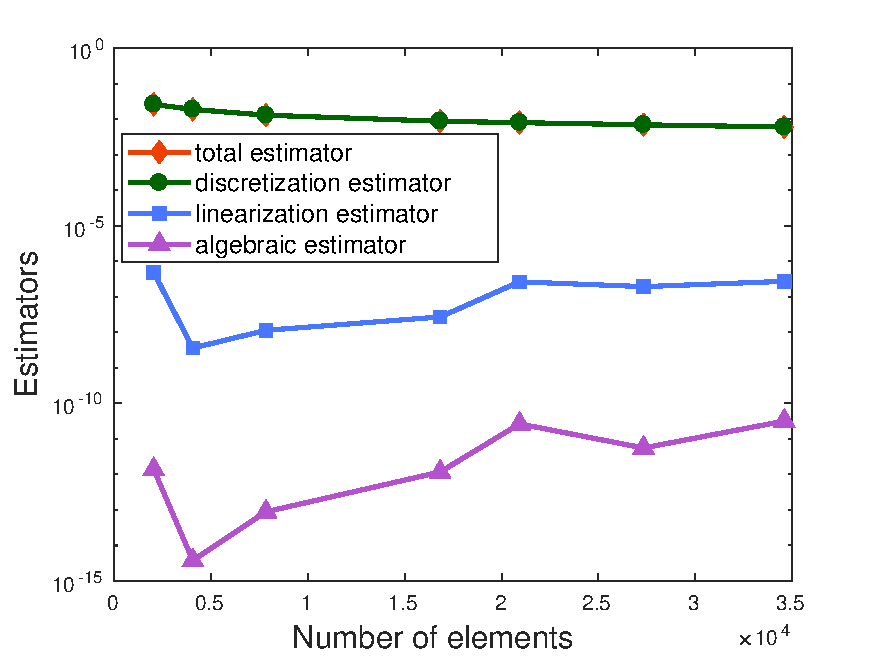
\includegraphics[width=\textwidth]{image_article_membrane_version_Juillet_2017/modif_exact_resolution_convergence_estimator_number_elements.eps}    
%\label{ref:position_membrane_convergence}
\end{minipage}\hfill
\begin{minipage}[c]{.33\linewidth}
   \centering
   Inexact Newton
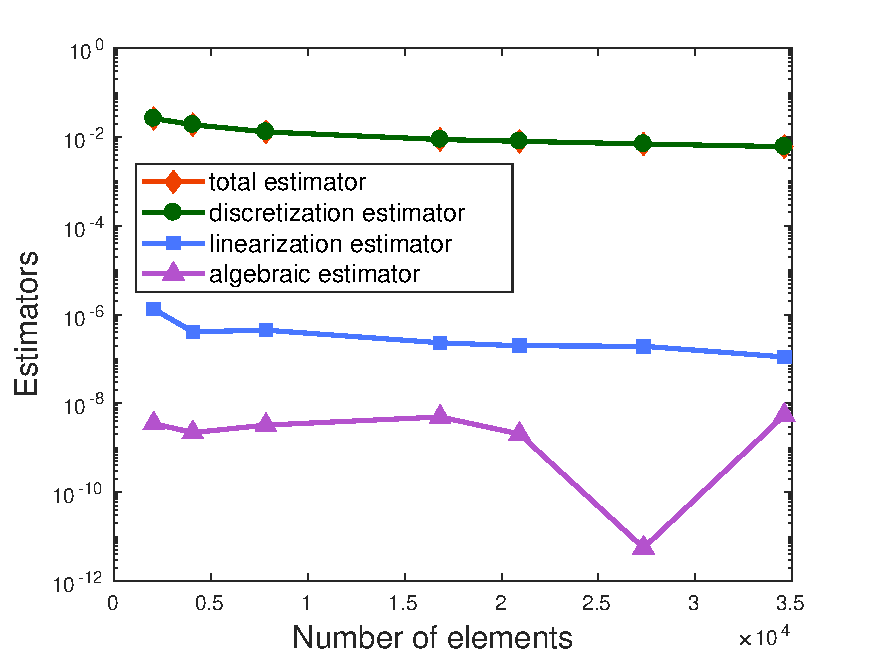
\includegraphics[width=\textwidth]{image_article_membrane_version_Juillet_2017/modif_inexact_resolution_convergence_estimator_number_elements.eps}    
%\label{ref:position_membrane_convergence}
\end{minipage}\hfill
\begin{minipage}[c]{.33\linewidth}
   \centering
   Adaptive inexact Newton
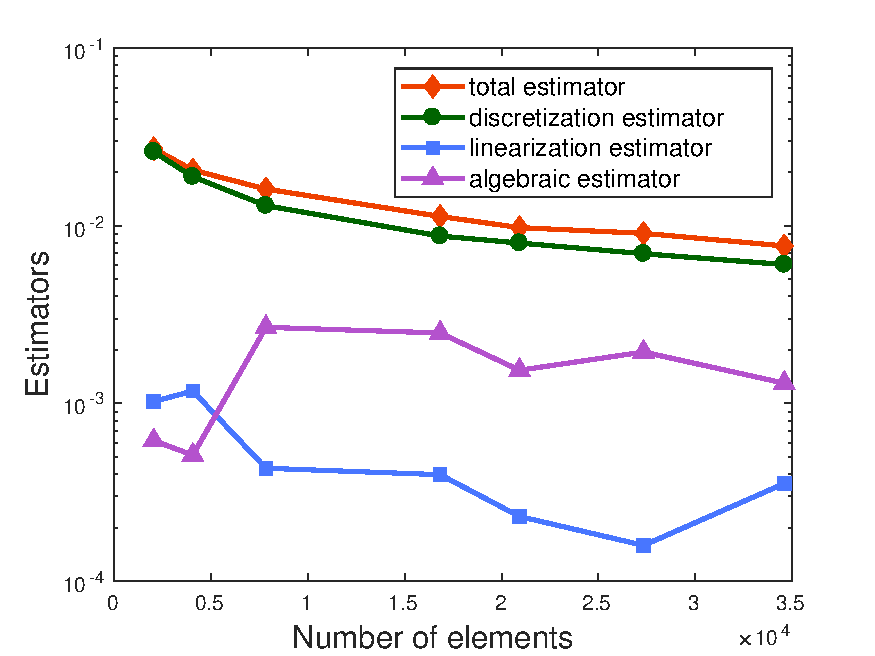
\includegraphics[width=\textwidth]{image_article_membrane_version_Juillet_2017/modif_adapt_inexact_resolution_convergence_estimator_number_elements.eps}     
%\label{ref:lambda_membrane_convergence} 
\end{minipage}
%\caption{Exact Newton(left), Inexact Newton(middle), adaptive inexact Newton(right)}
\end{figure}

\textcolor{red}{\textbf{Quality and precision are preserved for adaptive inexact semi-smooth Newton method.}}


\end{frame}

\begin{frame}
\begin{figure}
\begin{minipage}[c]{.33\linewidth}
   \centering
   Exact Newton
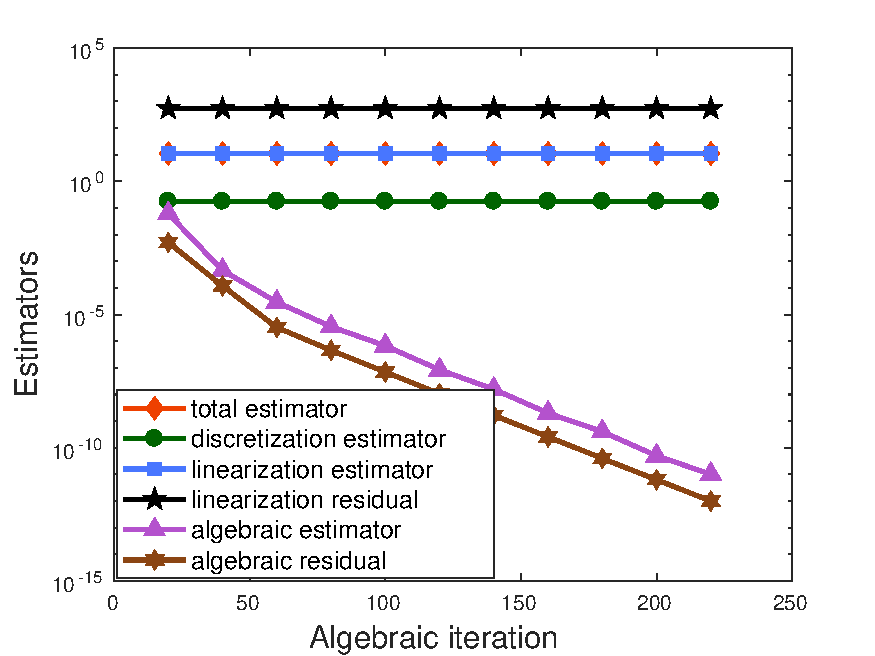
\includegraphics[width=\textwidth]{image_article_membrane_version_Juillet_2017/modif_exact_resolution_estimators_gmres_iter_inside_first_newton_iter_Hmax_015.eps}    
%\label{ref:position_membrane_convergence}
\end{minipage}\hfill
\begin{minipage}[c]{.33\linewidth}
   \centering
   Inexact Newton
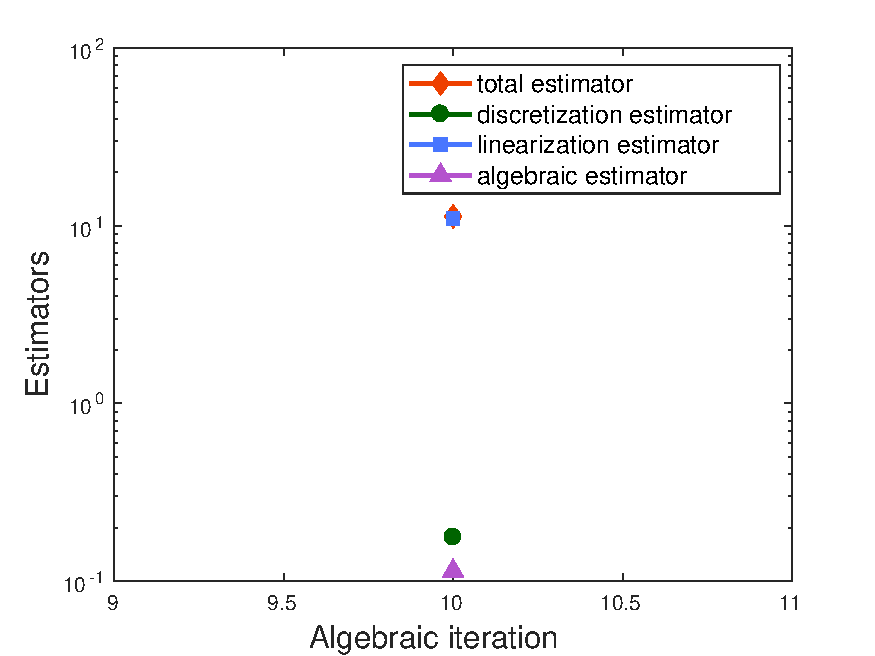
\includegraphics[width=\textwidth]{image_article_membrane_version_Juillet_2017/modif_inexacte_resolution_Hmax_015_number_gmres_iter_inside_first_newton_step.eps}    
%\label{ref:position_membrane_convergence}
\end{minipage}\hfill
\begin{minipage}[c]{.33\linewidth}
   \centering
   Adaptive inexact Newton
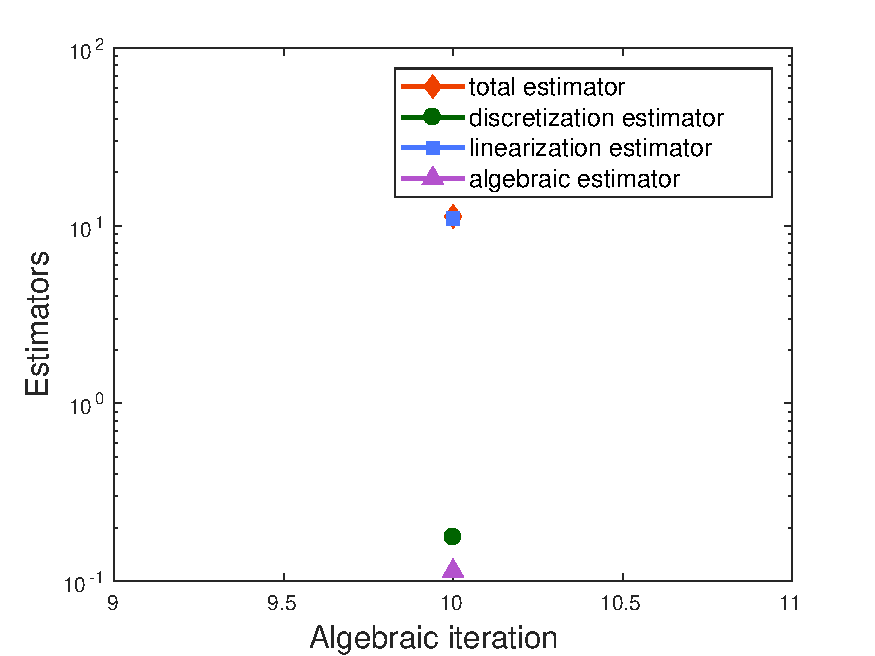
\includegraphics[width=\textwidth]{image_article_membrane_version_Juillet_2017/modif_adapt_inexact_resolution_estimators_gmres_iter_inside_first_newton_iter_Hmax_015.eps}     
%\label{ref:lambda_membrane_convergence} 
\end{minipage}
%\caption{Exact Newton(left), Inexact Newton(middle), adaptive inexact Newton(right)}
\end{figure}

\vspace{-0.3 cm}
\begin{figure}
   \begin{minipage}[c]{.33\linewidth}
   \centering
   Exact  Newton 
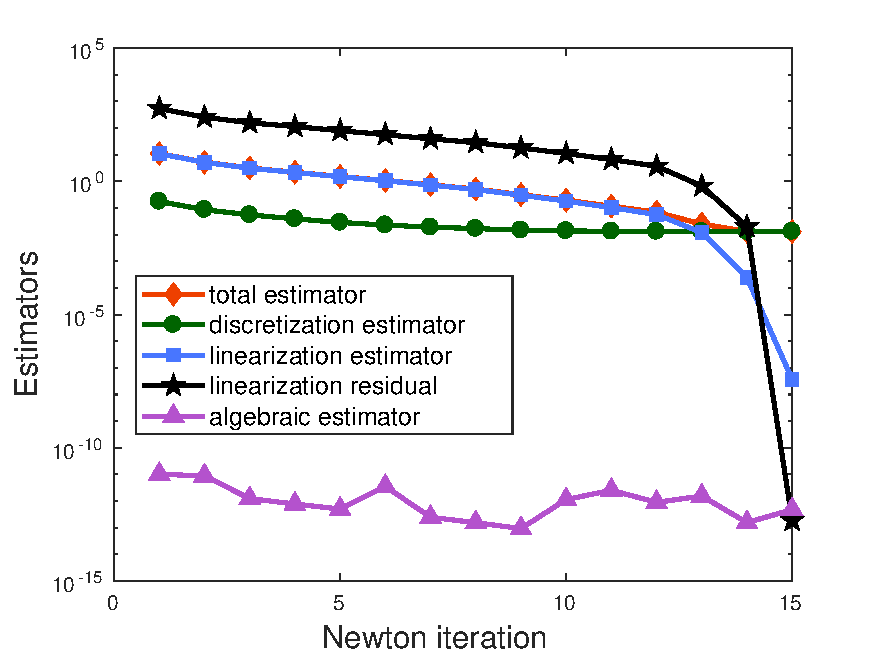
\includegraphics[width=\textwidth]{image_article_membrane_version_Juillet_2017/modif_exact_resolution_estimators_newton_iter_Hmax_015.eps}    
   \end{minipage} \hfill
   \begin{minipage}[c]{.33\linewidth}
   \centering
   Inexact Newton
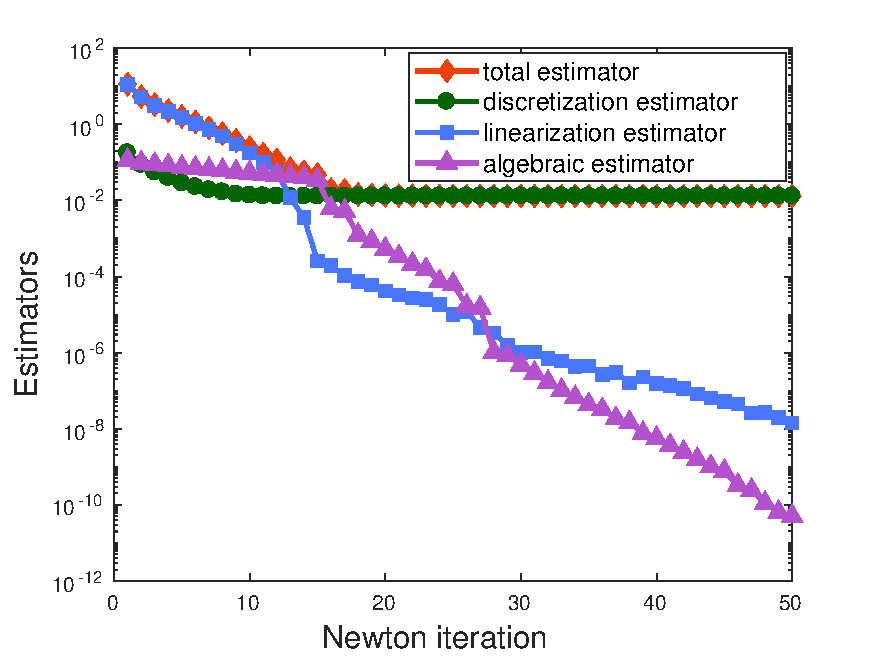
\includegraphics[width=\textwidth]{image_article_membrane_version_Juillet_2017/modif_inexacte_resolution_Hmax_015_estimators_newton_step.eps}     
   \end{minipage} \hfill
  \begin{minipage}[c]{.32\linewidth}
  \centering
  Adaptive Inexact Newton  
   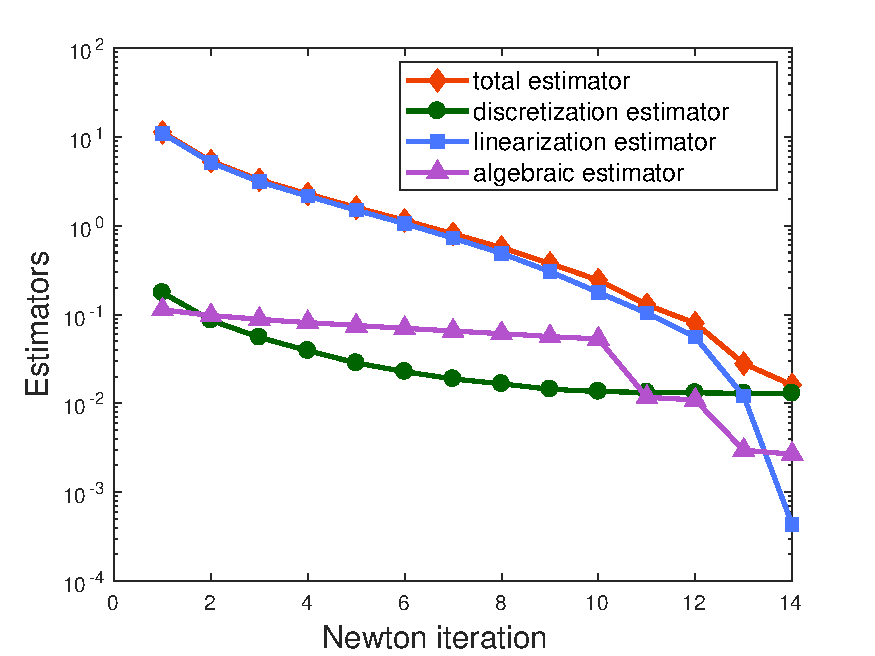
\includegraphics[width=\textwidth]{image_article_membrane_version_Juillet_2017/modif_adapt_inexact_resolution_estimators_newton_iter_Hmax_015.eps}     
\end{minipage}\hfill
\end{figure}
\end{frame}


%
%\begin{figure}[H]
%\begin{subfigure}[normal]{0.32\textwidth} 
%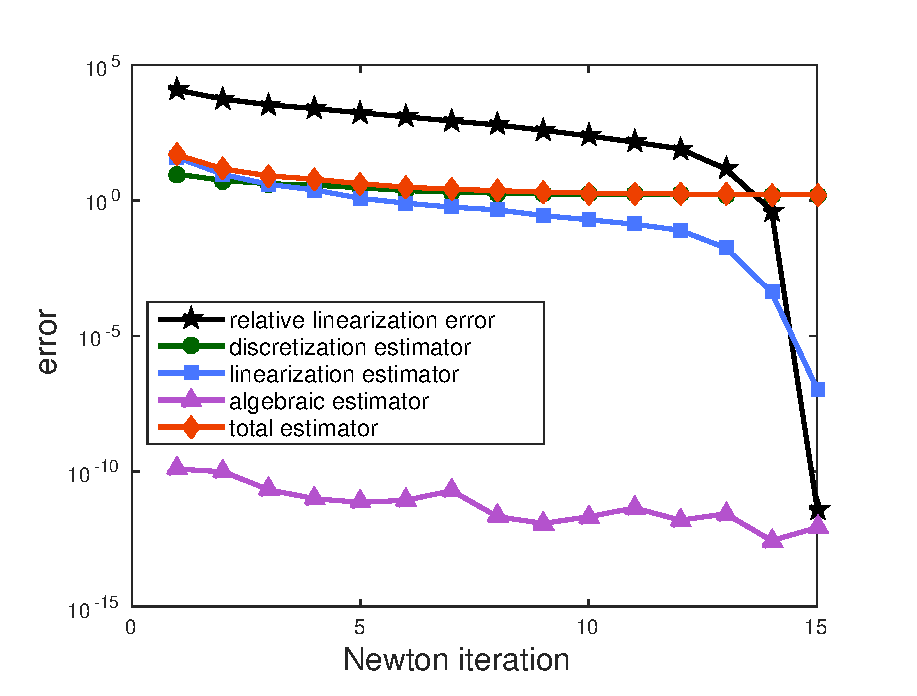
\includegraphics[width=\textwidth]{fig_article/estimators_newton_step_exact_resolution.eps}    
%%\label{ref:position_membrane_convergence}
%\end{subfigure}
%\begin{subfigure}[normal]{0.32\textwidth}
%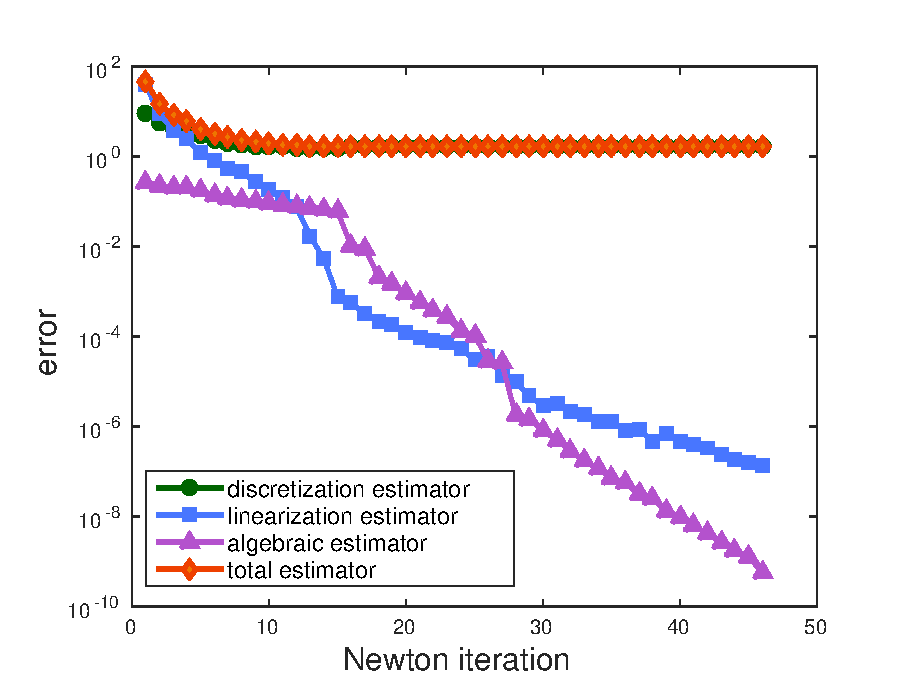
\includegraphics[width=\textwidth]{fig_article/estimators_newton_step_inexact_resolution.eps}     
%%\label{ref:lambda_membrane_convergence} 
%\end{subfigure}
%\begin{subfigure}[normal]{0.33\textwidth}
%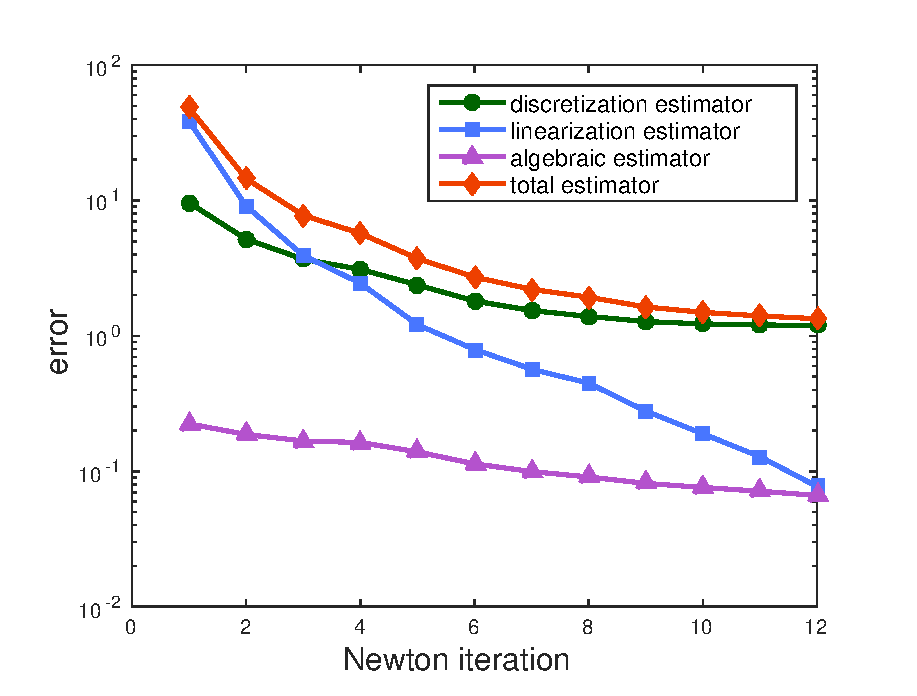
\includegraphics[width=\textwidth]{fig_article/estimators_newton_step_adapt_inexact_resolution.eps}     
%%\label{ref:lambda_membrane_convergence} 
%\end{subfigure}
%\caption{Exact Newton(left), inexact Newton(middle), adaptive inexacte Newton(right)}
%\end{figure}

\begin{frame}

%\begin{itemize}
%\item Effectivity indices as a function of the Newton iterations for 3 methods.
%\end{itemize}

\textcolor{red}{\textbf{Overall performance of the three approaches:}}
\begin{figure}[H]
\begin{minipage}[c]{.40\linewidth}
   \centering 
   Newton
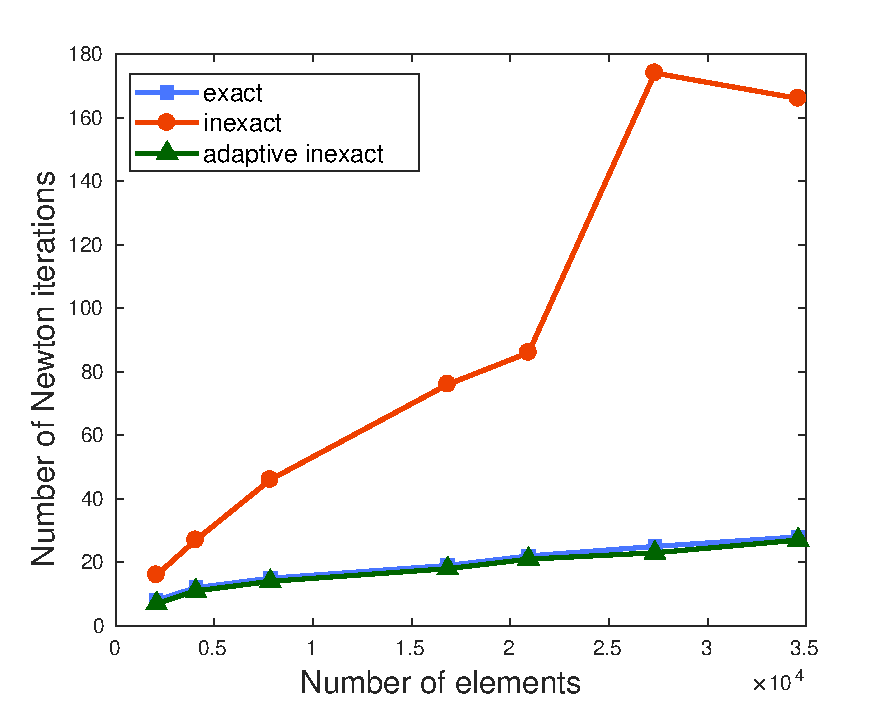
\includegraphics[width=\textwidth]{image_article_membrane_version_Juillet_2017/modif_comparison_three_methods_number_Newton_iter_number_elements.eps}    
%\label{ref:position_membrane_convergence}
\end{minipage}\hfill
\begin{minipage}[c]{.40\linewidth}
\centering
GMRES
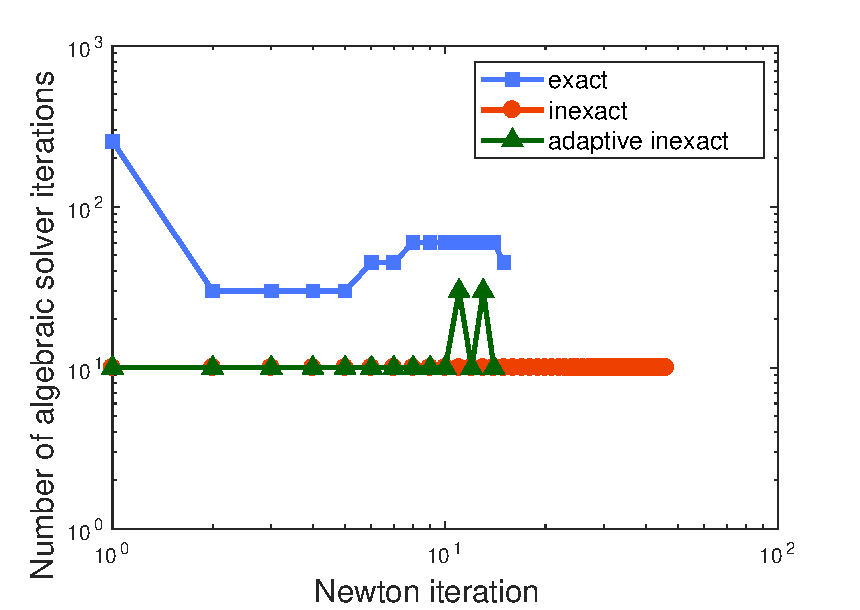
\includegraphics[width=\textwidth]{image_article_membrane_version_Juillet_2017/modif_comparison_three_methods_number_Gmres_iter_number_newton_step.eps}    
%\label{ref:position_membrane_convergence}
\end{minipage} \hfill
\end{figure}
\begin{figure}
\vspace*{-0.04\textwidth} \hspace*{0.1\textwidth}
\begin{minipage}{.40\linewidth} 
\centering   Total GMRES
 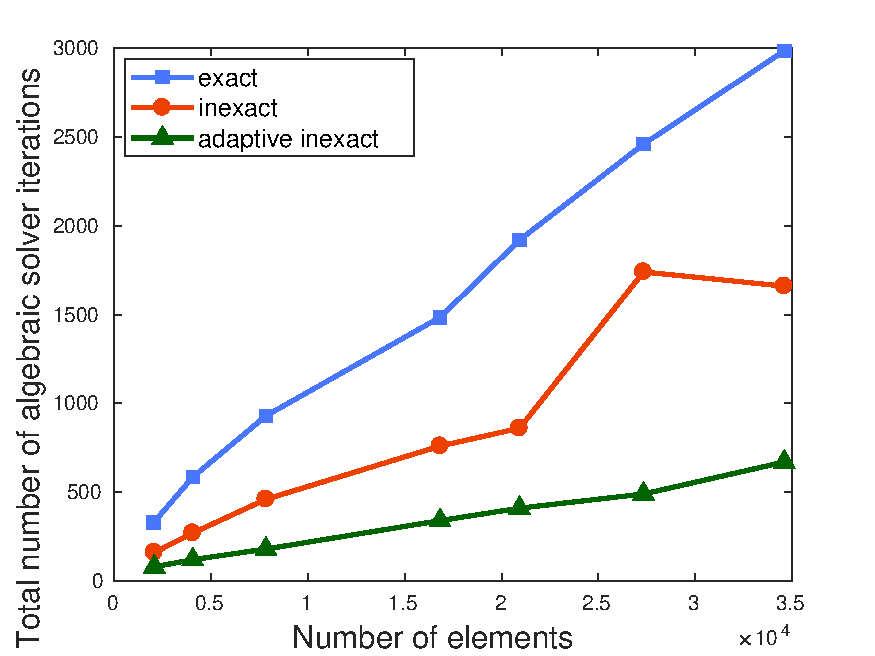
\includegraphics[width=\textwidth]{image_article_membrane_version_Juillet_2017/modif_comparison_three_methods_total_number_Newton_Gmres_iter_number_elements.eps}     
%\label{ref:lambda_membrane_convergence} 
\end{minipage} \hfill

%\caption{Number of Newton iterations per number of elements (left), number of linear solver iterations per Newton step, and total number of linear solver iterations per number of elements}
\label{ref:figure:plot:number:alg:iter:per:newton:step}
\end{figure}
\end{frame}
%\begin{frame}
%%\begin{figure}[H]
%\centering
%\begin{tabular}
%{|>{\begin{bf}} c <{\end{bf}}|c|c|c|c|c|}
%\hline
% $(\gamma_{\mathrm{alg}},\gamma_{\mathrm{lin}})$  & 
% $(0.1,0.1)$ &  $(0.01,0.1)$  & $(0.1,0.01)$ & $(0.01,0.01)$ \\
%\hline
% Newton iter &   21 &  21 &  25 &  25  \\
%\hline
% Algebraic iter ($k=5$) &   10 &  30 &  10 &  30\\
%\hline
% Total iter &   210 &  370 &  250 &  410 
%\label{ref:tableau:number:inex:adapt:iter_gamma:alg:0.1}
%%\caption{Adaptive inexact Newton method for a fixed mesh containing approximately 35000 elements and for several weights $\gamma_{\mathrm{alg}}$ and $\gamma_{\mathrm{lin}}$.}
%\label{ref:tableau:comparatif}
%
%\end{tabular}
%%\end{figure}
%\end{frame}

\begin{frame}
\begin{figure}
\begin{minipage}[c]{.38\linewidth}
   \centering
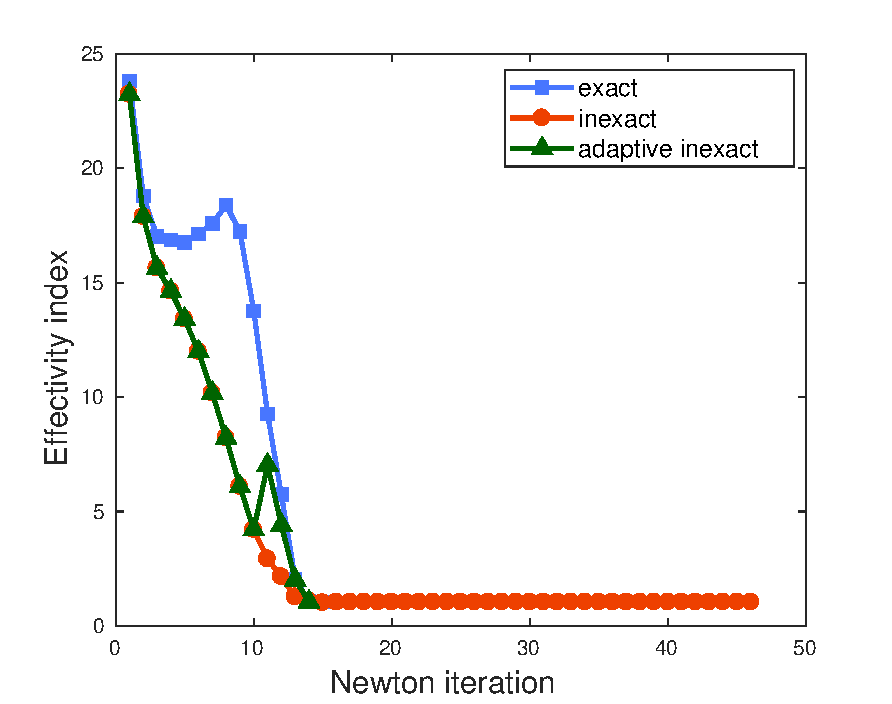
\includegraphics[width=\textwidth]{image_article_membrane_version_Juillet_2017/modif_effectivity_index_3_methods_Hmax_015.eps}    
%\label{ref:position_membrane_convergence}
\end{minipage}\hfill
\begin{minipage}[c]{.38\linewidth}
   \centering
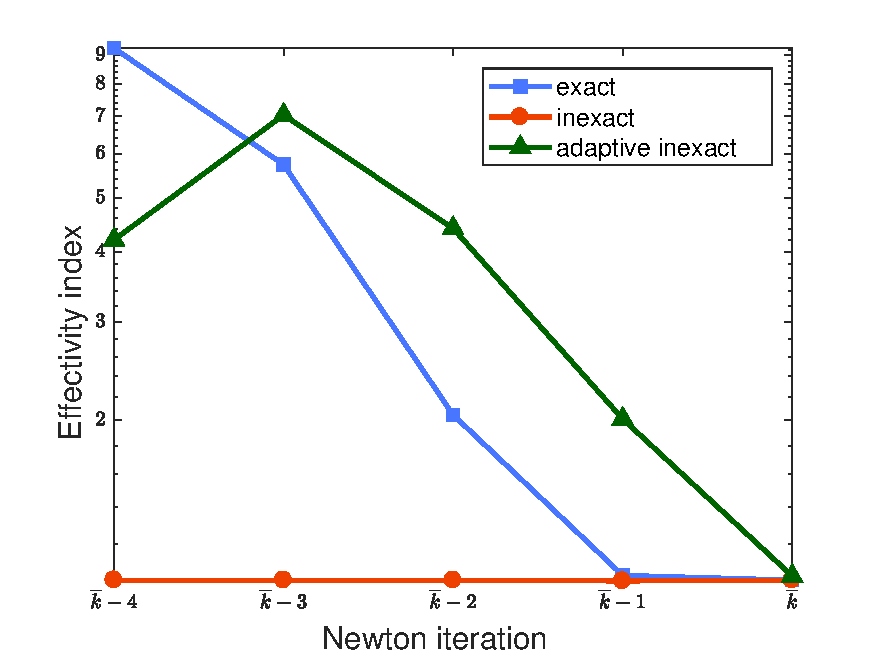
\includegraphics[width=\textwidth]{image_article_membrane_version_Juillet_2017/modif_effectivity_index_3_methods_last_newton_iter_Hmax_015.eps}     
%\label{ref:lambda_membrane_convergence} 
\end{minipage}\hfill
\end{figure}

\textcolor{red}{\textbf{Distribution of the error:}}
\begin{figure}[H]
\begin{minipage}[c]{.40\linewidth}
   \centering
   Actual error
\includegraphics[width=\textwidth]{fig_article/estimator_actual_error_inexact_newton_iter_30second_level_modif.eps}    
%\label{ref:position_membrane_convergence}
\end{minipage}\hfill
\begin{minipage}[c]{.40\linewidth}
   \centering
   Estimated error
\includegraphics[width=\textwidth]{fig_article/energy_norm_second_level_inexact_newton_iter_30_modif.eps}     
%\label{ref:lambda_membrane_convergence} 
\end{minipage}\hfill
%\caption{Estimated(left) and actual(right), $J=2$, inexact Newton}
\end{figure}



\end{frame}
\begin{frame}
\frametitle{Conclusion}
\begin{itemize}
\item
We devised an a posteriori error estimate between $\bu$ and $\uhki$ for a wide class of semi-smooth Newton methods.
\vspace{0.5 cm}

\item 
This estimate enables to control the error at each semi-smooth Newton step.
\vspace{0.5 cm}
\item
The adaptive inexact semi-smooth Newton method requires less non linear and linear steps. 
%\vspace{0.5 cm}
%\item We have adaptive stopping criteria for the discretization $h$, the semi-smooth Newton method $\textcolor{royalblue}{k}$ and for the linear algebra $\textcolor{burntorange}{i}$.
\vspace{0.5 cm}
\item
Extension of this work to  multiphase flow problem with exchange between phases (non linear complementarity conditions) in porous media.  
\end{itemize}
\vspace{1 cm}
\Large
\hspace{1.8 cm}
\textcolor{midnightblue}
{\textbf{
Thank you for your attention!}}
\end{frame}
%\begin{frame}
%\footnotesize
%\frametitle{Bibliography}
%\begin{itemize}
%\item
%Problem of contact between two membranes
%\end{itemize}
%\begin{thebibliography}{10}
%  \bibitem{VorBer:2008}
%Faker Ben~Belgacem, Christine Bernardi, Adel Blouza, and Martin
%  Vohral{\'{\i}}k.
%\newblock A finite element discretization of the contact between two membranes.
%\newblock {\em M2AN Math. Model. Numer. Anal.}, 43(1):33--52, 2008.
%\bibitem{VorBer:2012}
%Faker Ben~Belgacem, Christine Bernardi, Adel Blouza, and Martin
%  Vohral{\'{\i}}k.
%\newblock On the unilateral contact between membranes. {P}art 2: {\it a
%  posteriori} analysis and numerical experiments.
%\newblock {\em IMA J. Numer. Anal.}, 32(3):1147--1172, 2012.
%
%\end{thebibliography}
%\begin{itemize}
%\item
%Inexact Newton method and a posteriori adaptivity
%\end{itemize}
%\begin{thebibliography}{10}
%\bibitem{VorErn:2013}
%Alexandre Ern and Martin Vohral{\'{\i}}k.
%\newblock Adaptive inexact {N}ewton methods with a posteriori stopping criteria
%  for nonlinear diffusion {PDE}s.
%\newblock {\em SIAM J. Sci. Comput.}, 35(4):A1761--A1791, 2013.
%\end{thebibliography}
%
%\begin{itemize}
%\item
%Non smooth analysis and complementarity problem
%\end{itemize}
%\begin{thebibliography}{10}
%
%\bibitem{Facchinei:2003}
%Francisco Facchinei and Jong-Shi Pang.
%\newblock {\em Finite-dimensional variational inequalities and complementarity
%  problems. {V}ol. {I,II}}.
%\newblock Springer Series in Operations Research. Springer-Verlag, New York,
%  2003.
%
%%\bibitem{Pang:2003}
%%Francisco Facchinei and Jong-Shi Pang.
%%\newblock {\em Finite-dimensional variational inequalities and complementarity
%%  problems. {V}ol. {II}}.
%%\newblock Springer Series in Operations Research. Springer-Verlag, New York,
%%  2003.
%  \end{thebibliography}

%\end{frame}

%\begin{frame}
%\begin{center}
%{\Large \textbf {Thank you for your attention}}
%\end{center}
%\end{frame}
\bibliographystyle{plain}
\bibliography{biblio}
\end{document}
